%%%%%%%%%%%%%%%%%%%%%%%%%%%%%%%%%%%%%%%%
% BCS LaTeX template
% Version: 1.2
%%%%%%%%%%%%%%%%%%%%%%%%%%%%%%%%%%%%%%%%
\documentclass[a4paper, DIV=12, abstracton]{scrreprt}
\setcounter{secnumdepth}{5}
\setcounter{tocdepth}{5}


%%%%%%%%%%%%%%%%%%%%%%%%%%%%%%%%%%%%%%%%
% author and thesis details (please adjust accordingly)
%%%%%%%%%%%%%%%%%%%%%%%%%%%%%%%%%%%%%%%%
\newcommand{\name}{Gizem Ekinci} % <-- your name here
\title{Bayesian Inference of Information Transfer in Graph-Based Continuous-Time Multi-Agent Systems} % <-- thesis title here
\newcommand{\documenttype}{Master-Thesis} % <-- select type: "Master-Thesis", "Bachelor-Thesis", "Projektseminar", "Proseminar"
\newcommand{\major}{Elektro- und Informationstechnik} % <-- your study program
\newcommand{\supervisora}{Dipl.-Phys. Dominik Linzner}
\newcommand{\supervisorb}{Anam Tahir, M.Sc.}  % <-- your supervisor here
\newcommand{\submission}{21.07.2020} % <-- your submission date here
%%%%%%%%%%%%%%%%%%%%%%%%%%%%%%%%%%%%%%%%

%%% load document settings %%%
%%%%%%%%%%%%%%%%%%%%%%%%%%%%%%%%%%%%%%%%
% packages
%%%%%%%%%%%%%%%%%%%%%%%%%%%%%%%%%%%%%%%%

%%% math %%%
\usepackage{amsmath}
\usepackage{amssymb}
\usepackage{mathtools}
\usepackage{unicode-math}

%%% fonts %%%
\usepackage{lmodern}

%%% graphics %%%
\usepackage{tikz, wrapfig}
\graphicspath{{figures/}}
\usepackage{subcaption}
\usepackage{float}
\usepackage{graphicx}
\usetikzlibrary{positioning}
\usetikzlibrary{arrows}

%%% bibliography %%%
\bibliographystyle{plain}
\usepackage{etoolbox}
\AtBeginEnvironment{thebibliography}{\interlinepenalty=10000}

%%% misc %%%
\usepackage{blindtext}

%%% algorithms %%%
\usepackage{algorithmic}
\usepackage[ruled, lined, longend]{algorithm2e}

%%% referencing %%%
\usepackage[bookmarks, bookmarksdepth=chapter, hidelinks]{hyperref}
\usepackage[capitalise, noabbrev]{cleveref}
\newcommand{\crefrangeconjunction}{-}
\usepackage{xr}


%%%%%%%%%%%%%%%%%%%%%%%%%%%%%%%%%%%%%%%%
% document settings
%%%%%%%%%%%%%%%%%%%%%%%%%%%%%%%%%%%%%%%%

%%% title page %%%
\author{}
\date{}
\titlehead{
	\centering
	
\includegraphics[width=10cm]{tud_logo.pdf} \\
	\large\sffamily
	Fachbereich Elektrotechnik und Informationstechnik \\
	Bioinspired Communication Systems
	\vspace{10ex}
} 
\subtitle{
	\vspace{2ex}
	\documenttype\\
	\normalfont \sffamily 
	\major \\
	\vspace{4ex}
	Eingereicht von\\
	\vspace{2ex}
	{\Large \name}\\
	\vspace{2ex}
	am\\
	\submission\\
	\vspace{4ex}
	\parbox{0cm}{%
	\begin{tabbing}
	1.~Gutachten: \= Prof.~Dr.~techn.~Heinz~Koeppl \\
	2.~Gutachten: \>\supervisora \\
	3.~Gutachten: \>\supervisorb
	\end{tabbing}}
}

%%% paragraph settings %%%
\parindent0ex
\parskip\baselineskip



%%%%%%%%%%%%%%%%%%%%%%%%%%%%%%%%%%%%%%%%
% commands
%%%%%%%%%%%%%%%%%%%%%%%%%%%%%%%%%%%%%%%%

%%% probability %%%
\newcommand{\given}{\,|\,}
\newcommand{\p}{p}

\DeclareRobustCommand{\rchi}{{\mathpalette\irchi\relax}}
\newcommand{\irchi}[2]{\raisebox{\depth}{$#1\chi$}}
\DeclareMathOperator*{\argmax}{arg\,max}
\DeclareMathOperator*{\argmin}{arg\,min}

\RedeclareSectionCommands[
	beforeskip=-3.25ex plus -1ex minus -0.2ex,
	runin=false,
	afterskip=2sp
]{paragraph,subparagraph}


\begin{document}
	\maketitle
	\pagestyle{empty}\ \newpage

\paragraph*{Erkl\"arung zur Abschlussarbeit gem\"a\ss~$\boldsymbol{\S}$22 Abs.~7 und $\boldsymbol{\S}$23 Abs.~7 APB TU Darmstadt}\ \\[\baselineskip]
Hiermit versichere ich, \name, die vorliegende Arbeit gem\"a\ss~\S 22 Abs.~7 APB der TU Darmstadt ohne Hilfe Dritter und nur mit den angegebenen Quellen und Hilfsmitteln angefertigt zu haben. Alle Stellen, die Quellen entnommen wurden, sind als solche kenntlich gemacht worden. Diese Arbeit hat in gleicher oder \"ahnlicher Form noch keiner Pr\"ufungsbeh\"orde vorgelegen. Mir ist bekannt, dass im Falle eines Plagiats (\S38 Abs.2 APB) ein T\"auschungsversuch vorliegt, der dazu f\"uhrt, dass die Arbeit mit 5,0 bewertet und damit ein Pr\"ufungsversuch verbraucht wird. Abschlussarbeiten d\"urfen nur einmal wiederholt werden. Bei der abgegebenen Arbeit stimmen die schriftliche und die zur Archivierung eingereichte elektronische Fassung gem\"a\ss\ \S 23 Abs.~7 APB \"uberein.\\

English translation for information purposes only:\\[\baselineskip]
Thesis statement pursuant to \S22 paragraph 7 and \S23 paragraph 7 of APB TU Darmstadt:\\
I herewith formally declare that I, \name, have written the submitted thesis independently pursuant to \S22 paragraph 7 of APB TU Darmstadt. I did not use any outside support except for the quoted literature and other sources mentioned in the paper. I clearly marked and separately listed all of the literature and all of the other sources which I employed when producing this academic work, either literally or in content. This thesis has not been handed in or published before in the same or similar form.
I am aware, that in case of an attempt at deception based on plagiarism (§38 Abs. 2 APB), the thesis would be graded with 5,0 and counted as one failed examination attempt. The thesis may only be repeated once. In the submitted thesis the written copies and the electronic version for archiving are pursuant to § 23 paragraph 7 of APB identical in content.\\


Darmstadt, den \submission\\

\rule{6cm}{0.7pt}\\
(\name)

	\newpage \
\newpage

\begin{abstract}
	Multi-agent systems in nature, such as a population of cells, cooperate through information sharing. This information can be incomplete and noisy. Inspired by such systems, we consider communication between three individuals, which are evolving continuously in time. Two of them act independently, and emit messages containing information about their states, while the third one receives a translation of these messages. Based on these translated observations, the agent node forms its belief over the state of other nodes. We modelled this system combining continuous-time Bayesian network (CTBN) and partially observable Markov decision (POMDP) process frameworks. The nodes evolve continuously in time as components of a CTBN. Given that the true messages are unavailable to the agent, the interaction between the nodes is modelled as POMDP. The exact update of the belief state is computed by filtering, and these results are used as a baseline. The approximation of the belief state is obtained using marginalized particle filtering. This work aims to infer the language model which leads to the translations.\\
	%The belief state is updated utilising two methods. The first one is exact update, discussed in \cref{par:bs_exact}, and assumes that the transition intensities of the parents $ \textbf{Q}_1 $ and $ \textbf{Q}_2 $ are available both for the agent and for the classifier. However, due to the fact that this would not present a realistic system, particle filtering with marginalized CTBN is introduced for as state estimator. Here, both the agent and the classifier was able to perform the belief state update, given Gamma-priors of $ \textbf{Q}_1 $ and $ \textbf{Q}_2 $.\\
\end{abstract}

\newpage \
\newpage
	
	\pagenumbering{gobble}
	\tableofcontents
	\newpage
	\setcounter{page}{1}
	\pagenumbering{roman}
	\chapter*{List of Symbols}
\addcontentsline{toc}{chapter}{List of Symbols}

\begin{tabular}{cp{0.6\textwidth}}
	$ X(t) $ & value of stochastic process $X$ at time t \\
	$ X^{[0, T]} $ & discrete valued trajectory of stochastic process $ X $ in time interval $ [0, T] $ \\
	$x$ & position \\
	$v$ & velocity \\
	$a$ & acceleration \\
	$t$ & time \\
	$F$ & force
\end{tabular}\\

	\listoffigures
	\addcontentsline{toc}{chapter}{List of Figures}
	\newpage
	\setcounter{page}{1}
	\pagenumbering{arabic}
	\pagestyle{plain}
	
	\chapter{Introduction}

\blindtext

\section{Problem Statement}

\blindtext

\section{Related Work}

\blindtext

\section{Contributions}

\blindtext
	\newpage \ \thispagestyle{empty} \addtocounter{page}{-1}
	\chapter{Foundations}
\label{chap:2}

This chapter presents the theory applied in this thesis. First, the details of the communication problem is described briefly to put the theory into perspective, and then the mathematical theory of the frameworks used to model this problem is introduced. 

\section{Problem Formulation}
\label{sec:prob_formulation}
\begin{wrapfigure}{r}{3.5cm}
	\begin{center}
		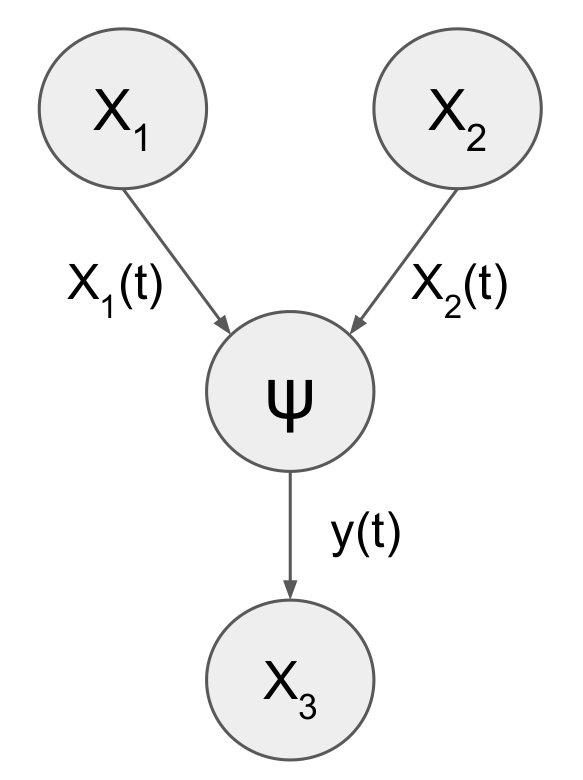
\includegraphics[width=3.5cm]{figures/simple_graph}
		\caption{Communication model.}
	\end{center}
	\label{fig:graph_model}
\end{wrapfigure} 
The communication model considered in this thesis is given in \autoref{fig:graph_model}. The parent nodes, $X_{1}$ and $ X_{2}$, emit messages which carry information about their states. These messages are translated by an observation model, $\psi$, and agent node, $ X_{3} $ makes a decision based on this translated message, $ y $. The main objective is to infer the observation model given set of trajectories of nodes.

The transition models of the nodes and the dependencies between them are modelled as continuous-time Bayesian network (CTBN), denoted by \textbf{X}. The network \textbf{X} represents a stohastic process over a structured multivariate state space $ \rchi = [\rchi_1,..., \rchi_n] $. 

The messages that are emitted by the parent nodes $X_{1}$ and $ X_{2} $ are modelled as independent homogeneous continuous-time Markov processes $X_{i}(t)$, with state space $ \rchi_{i} = \left\lbrace x_{1}, x_{2}, ..., x_{n} \right\rbrace  $ for $ i \in \left\lbrace 1,2 \right\rbrace $.

The agent node $ X_3 $ does not have a direct access to the messages, but observes a translation of them. The observation model is defined as the likelihood of a translation given the parent messages.
\begin{equation}
\psi \coloneqq p(y(t) \mid X_{1}(t), X_{2}(t))
\end{equation}
The agent  $ X_{3} $ is modelled as inhomogenouos continuous-time Markov process with state space $ \rchi_{3} = \left\lbrace x_{1}, x_{2}, ..., x_{n} \right\rbrace  $ and set of actions $ a \in \left\lbrace a_{0}, a_{1}, ..., a_{k}\right\rbrace  $ to choose from. 

Given the observation, the agent forms a belief over the parent states, $  b(x_{1}, x_{2}; t) $, that summarizes the past observations.\cite{KAELBLING199899} The policy of the agent, $ \pi(a \mid b) $, is assumed to be shaped by evolution (close) to optimality. Based on the belief state, the agent takes an action, which in the setting described above means to change its internal dynamics. 
\section{Continuous Time Bayesian Networks}
A continuous-time Bayesian network (CTBN) is a graphical model that represents a collection of nodes whose values evolve continuously over time. In CTBN framework, through a directed graph, the dependencies of a set of Markov processes (MPs) can be modelled efficiently relying on two assumptions. First assumption is that only one node can transition at a time. Secondly, the instantenous dynamics of each node depends only on its parent nodes. \cite{Cohn2010a, Nodelman1995} 
%In the following, every node of a CTBN is considered to be a Markov process.
\subsection{Continuous Time Markov Processes}
A continuous-time Markov process (CTMP) is a continuous-time stochastic process which satisfies Markov property, namely, the probability distribution over the states at a future time is conditionally independent of the past states given the current state.\cite{Cohn2010a} Let X be a CTMP with state space $ \rchi = \left\lbrace x_{1}, x_{2}, ..., x_{n} \right\rbrace  $. Then the Markov property can be written as follows:
\begin{equation}
	\operatorname{Pr}\left(X^{\left(t_{k}\right)}=x_{t_{k}} | X^{\left(t_{k-1}\right)}=x_{t_{k-1}}, \ldots, X^{\left(t_{0}\right)}=x_{t_{0}}\right)=\operatorname{Pr}\left(X^{\left(t_{k}\right)}=x_{t_{k}} | X^{\left(t_{k-1}\right)}=x_{t_{k-1}}\right)
\end{equation}
A CTMP is represented by its transition intensity matrix, $ \textbf{Q} $. In this matrix, the intensity $ q_{i} $ represents the instantaneous probability of leaving state $ x_{i} $ and $ q_{i,j} $ represents the instantaneous probability of switching from state $ x_{i} $ to $ x_{j} $. 
\begin{equation}
	\textbf{Q} = 
	\begin{bmatrix}
	-q_{1} & q_{1,2} & 	{\hdots}  & q_{1,n} \\
	q_{2,1} & -q_{2} & 	{\hdots}  & q_{2,n}  \\
	{\vdots}  & 	{\vdots}  & 	{\ddots}  & {\hdots}  \\
	q_{n,1} &  q_{n,2} &  {\hdots} & -q_{n}
	\end{bmatrix}
\label{eq:Q_matrix}
\end{equation}
where $ q_{i} = \sum_{i \neq j} q_{i,j}$.\cite{Nodelman1995}

\subsubsection{Homogenous Continuous Time Markov Processes}
A continuous-time Markov process is time-homogenous when the transition intensities do not depend on time. Let X be a homogenous CTMP, with transition intensity matrix $ \textbf{Q}_X $. Infinitesimal transition probability from state $ x_{i} $ to $ x_{j} $ in terms of the transition intensities $ q_{i,j} $ can be written as \cite{Cohn2010a}:
\begin{equation}
p_{i,j}(h)=\delta_{ij}+q_{i,j} h+o(h)
\label{eq:Markov_trans_func}
\end{equation}
where $ p_{i, j}(h) \equiv Pr(X(t+h)=x_j\mid X(t)=x_i) $ are Markov transition functions, $ \delta_{i,j} = \delta(x_i,x_j)$ is Kronecker delta and o(.) is a function decaying to zero faster than its argument.

The \textit{master equation} is then derived as follows:
\begin{align}
	p_{j}(t) &= \operatorname{Pr}(X(t) = x_{j}) \nonumber\\
		& =\sum_{\forall i} p_{i, j}(h) p_{i}(t-h) \nonumber \\
	\lim_{h\rightarrow 0} p_{j}(t) 
		& = \lim_{h\rightarrow 0} \sum_{\forall i} \left[ \delta_{ij}+q_{i,j} h+o(h)\right]  p_{i}(t-h) \nonumber \\ 
		& = \lim_{h\rightarrow 0} p_{j}(t-h) + \lim_{h\rightarrow 0} h \sum_{\forall i} q_{i,j} p_{i}(t-h) \nonumber \\
	\lim_{h\rightarrow 0} \frac{p_{j}(t) - p_{j}(t-h)}{h} 
		&= \lim_{h\rightarrow 0} \sum_{\forall i} q_{i,j} p_{i}(t-h) \nonumber\\
	\frac{d}{dt} p_{j}(t) & = \sum_{\forall i} q_{i,j} p_{i}(t)
%		& = \sum_{\forall i \neq j}\left[  q_{i,j} p_{i}(t) - q_{j,i} p_{j}(t) \right]\nonumber
	\label{eq:master_equation}
\end{align}
Equation \ref{eq:master_equation} can be written in matrix form:
\begin{equation}
\frac{d}{dt} p(t) = p(t)\textbf{Q}
\end{equation}
where the time-dependent probability distribution $ p(t) $ is a row vector with entries $ {p_{i}(t)}_{x_{i}\in \rchi} $. 
The solution of this ODE is, 
\begin{equation}
p(t)=p(0) \exp (t\textbf{Q})
\end{equation}
with initial distribution $ p(0) $.

The amount of time staying in a state $ x_{i} $ is exponentially distributed with parameter $ q_{i} $. The probability density function $ f $ and cumulative distribution function $ F $ for staying in the state $ x_{i} $ \cite{Nodelman1995}:
\begin{align}
f(t) & = q_{i} \exp \left(-q_{i} t\right), t\geq 0  \label{eq:f(t)_homo}\\
F(t) & = 1 - \exp \left(-q_{i} t\right), t\geq 0 
\end{align}
Given the transitioning from state $ x_{i} $, the probability of landing on state $ x_{j} $ is $ q_{i,j}/q_{i} $.
\paragraph*{Likelihood Function}
\label{sec:llh_of_homo}
Consider a single transition denoted as $ d = <x_{i},x_{j},t> $, where transition occurs from state $ x_{i} $ to $ x_{j} $ after spending t amount of time at state $ x_{i} $. The likelihood of this transition is the product of the probability of having remained at state $ x_{i} $ for that long, and the probability of transitioning to $ x_{j} $.
\begin{equation}
\operatorname{Pr}(d  \mid \textbf{Q}) = \left( q_{i}exp(-q_{i}t) \right) \left( \frac{q_{i,j}}{q_{i}} \right)
\end{equation}
The likelihood of a trajectory sampled from a homogenous CTMC, $ X^{[0,T]} $, can be decomposed as the product of the likelihood of single transitions. The sufficient statistics summarizing this trajectory can be written as $ T[x_{i}] $, total amount of time spent in state $ x_{i} $, $ M[x_{i}, x_{j}] $ total number of transitions from state $ x_{i} $ to $ x_{j} $. Then the likelihood of a trajectory $  X^{\left[0,T\right] } $ can be written as:
\begin{align}
\operatorname{Pr}(X^{[0,T]}  \mid \textbf{Q}) &=  \prod_{d \in X^{[0,T]}} \operatorname{Pr}(d \mid \textbf{Q}) \nonumber\\&=\left(\prod_{ i} q_{i}^{M[x_{i}]} \exp \left(-q_{i} T[x_{i}]\right)\right)\left(\prod_{ i} \prod_{ j \neq i} \left(\frac{q_{i,j}}{q_{i}}\right)^{M\left[x_{i}, x_{j}\right]}\right) \nonumber\\ & = \prod_{j \neq i}  exp(-q_{i,j}T[x_{i}])\ q_{i,j}^{M[x_{i},x_{j}]}
\label{eq:lh_traj_homo}
\end{align}
where $ M[x_{i}] = \sum_{j \neq i} M[x_{i}, x_{j}] $ is the total number transitions leaving state $ x_{i} $.


\subsubsection{Conditional Markov Processes}
A continuous-time Markov process is \textit{time-inhomogenous} when the transition intensities changes over time. In a CTBN, while every node is a Markov process, the leaf nodes are characterized as \textit{conditional} Markov processes, a type of inhomogeneous MP, where the intensities change over time, but not as a function of time rather as a function of parent states. \cite{Nodelman1995} 

Let X be a conditional Markov process, with a set of parents $ \textbf{U} = Par(X)$. Its intensity matrix, \textit{conditional intensity matrix}, $ \textbf{Q}_{X\given \textbf{U}} $ can be viewed as a set of homogenous intensity matrices $ \textbf{Q}_{X\given \textbf{u}} $, with entries $ q_{i,j \mid \textbf{u}} $ (similar to \autoref{eq:Q_matrix}), for each instantiation of parent nodes $ \textbf{U}(t) =\textbf{u} $.\cite{Nodelman1995} As a result, given a trajectory of parent nodes, X has a trajectory of intensity matrix as a combination of these homogenous matrices.
\begin{equation}
\textbf{Q}^{[0,T]} = [\textbf{Q}_{X\given \textbf{U}(t_0)}, \textbf{Q}_{X\given \textbf{U}(t_1)}, ..., \textbf{Q}_{X\given \textbf{U}(t_N)}],\ 0<t_0<t_1<...<t_N\leq T
\end{equation}

Markov transition function for a conditional Markov process can be written as follows:
\begin{align}
\operatorname{Pr}(X(t + h) = x_j \mid X(t)=x_i, \textbf{U}(t)=u, \textbf{Q}_{X\given \textbf{u}}) = \delta(i,j) + q_{i,j \mid \textbf{u}} h + o(h)
\label{eq:CIM_trans_funct}
\end{align}


\paragraph*{Likelihood Function}
Given the instantiation of its parents, the complete information on the dynamics of X is obtained. Then the likelihood of a trajectory drawn from a conditional MP $ X $ can be written similar to \autoref{eq:lh_traj_homo},
\begin{align}
\operatorname{Pr}(X^{[0,T]}  \mid \textbf{Q}_{X\given \textbf{U}}) &=  \left(\prod_{ \textbf{u}}\prod_{ i} q_{i\mid \textbf{u}}^{M[x_{i}\mid \textbf{u}]} \exp \left(-q_{i\mid \textbf{u}} T[x_{i}\mid \textbf{u}]\right)\right)\left(\prod_{ \textbf{u}}\prod_{ i} \prod_{ j \neq i} \left(\frac{q_{i,j\mid \textbf{u}}}{q_{i\mid \textbf{u}}}\right)^{M\left[x_{i}, x_{j}\mid \textbf{u}\right]}\right) \nonumber\\ & = \prod_{ \textbf{u}}\prod_{j\neq i}  exp(-q_{i,j\mid \textbf{u}}T[x_{i}\mid \textbf{u}]) \ q_{i,j\mid \textbf{u}}^{M[x_{i},x_{j}\mid \textbf{u}]}
\label{eq:lh_traj_cond}
\end{align}
with the sufficient statistics introduced in \autoref{sec:llh_of_homo} are also conditioned on parent nodes.
%Let X be an inhomogeneous Markov process. $  X^{\left[0,T\right] } $ is a trajectory sampled from this process with $ m $ number of transitions, $ 0 = t_{0} < t_{1} < ... < t_{m} $ are the times where transition occurred, and $ x_{t_{0}}, x_{t_{1}},..., x_{t_{m}} $ are the observed states. The likelihood of trajectory  $  X^{\left[0,T\right] } $ can be written as follows: 
%\begin{equation}
%\operatorname{Pr}(X^{[0,T]}  \mid \textbf{Q}) = \prod_{k=1}^{m} \left[ q_{x_{k-1}} (t_{k}) \exp \left(-\int_{t_{k-1}}^{t_{k}} q_{x_{k-1}}(u) d u\right) \frac{q_{x_{k-1}, x_{k}} (t_{k})}{q_{x_{k-1}}(t_{k})}\right] 
%\label{eq:lh_traj_inhomo}
%\end{equation}
%For inhomogeneous CTMP, Equation \ref{eq:f(t)_homo} becomes:
%\begin{equation}
%f(t) = q_{i}(t) \exp \left(-\int_{0}^{t} q_{i}(u) d u\right)
%\end{equation}
%Let X be an inhomogeneous Markov process. $  X^{\left[0,T\right] } $ is a trajectory sampled from this process with $ m $ number of transitions, $ 0 = t_{0} < t_{1} < ... < t_{m} $ are the times where transition occurred, and $ x_{t_{0}}, x_{t_{1}},..., x_{t_{m}} $ are the observed states. The likelihood of trajectory  $  X^{\left[0,T\right] } $ can be written as follows: 
%\begin{equation}
%\operatorname{Pr}(X^{[0,T]}  \mid \textbf{Q}) = \prod_{k=1}^{m} \left[ q_{x_{k-1}} (t_{k}) \exp \left(-\int_{t_{k-1}}^{t_{k}} q_{x_{k-1}}(u) d u\right) \frac{q_{x_{k-1}, x_{k}} (t_{k})}{q_{x_{k-1}}(t_{k})}\right] 
%\label{eq:lh_traj_inhomo}
%\end{equation}


\subsection{The CTBN Model}
Evidently, a homogenouos CTMP can be considered as a conditional MP whose set of parents is empty. Thus, a CTBN can be formed as a set of conditional Markov processes.

Let \textbf{X} be a CTBN with local variables $ X_n $, $ n \in \left\lbrace 1,...N \right\rbrace $, each with a state space $ \rchi_n $. Given the dependencies of each variable as set of its parents $ \textbf{U}_n = Par(X_n) $, the transition model of each local variable $ X_n $ is modelled as conditional Markov processes. \cite{Nodelman1995} In the following the set of all conditional transition intensity matrices are denoted as $ \textbf{\textit{Q}} $.

Consider a trajectory drawn from CTBN $ \textbf{X} $, such that $ \textbf{X}^{[0, T]} = \left\lbrace X_1^{[0,T]},  X_2^{[0,T]}, ...,  X_N^{[0,T]}\right\rbrace  $. Following \autoref{eq:lh_traj_cond}, the likelihood of this trajectory can be written as follows.
\begin{align}
\operatorname{Pr}( \textbf{X}  | \textbf{\textit{Q}} ) = \prod_{n=1}^{N} \prod_{\textbf{u} \in \mathcal{\textbf{U}}_{n}} \prod_{x_i \in \mathcal{X}_{n}} \prod_{x_j \in \mathcal{X}_{n} \backslash x_i}
\exp \left[q_{i,j\mid \textbf{u}}^{n} T_{n}[x_i\mid \textbf{u}]\right] (q_{i,j\mid \textbf{u}}^{n})^{M_{n}[x_i, x_j\mid \textbf{u}]}
\end{align}
where $ T_n[.] $ and $ M_n[.] $ indicates the sufficient statistics for $ X_n $

\section{Belief State in Partially Observable Markov Decision Processes}
\label{sec:belief_POMDP}
Partially observable Markov decision process (POMDP) framework provides a model of an agent which interacts with its environment, but unable to obtain certain information about its state. Instead, the agent gets an observation which is a stochastic function of the true state. The main goal, as similar to Markov decision processes (MDPs), is to learn a policy solving a task by optimizing a reward function. The problem of decision making under uncertainty can be decomposed into two parts for the agent. The first is \textit{state estimator} to keep a belief state which is a sufficient statistic of its past experiences, and the second is the \textit{optimal policy} which will give an action based on the belief state. \cite{Murphy2000,KAELBLING199899}

In the problem considered in this thesis, the agent node $ X_{3} $ cannot observe the incoming messages directly, rather a summary of them. This presents a POMDP problem. However, since the optimal policy of the agent is assumed to be given, the theory for policy optimization is skipped. In this section, update methods for belief state is introduced.

In the following, belief state refers to the posterior probability distribution over the environment states.

\subsection{Exact/Bayes(?) Belief State Update}
\label{sec:exact_update}
Consider a POMDP problem, with discrete state space \textit{S}, action space \textit{A}, observation space $ \Omega $. In a scneario where a compact representation of the \textit{transition model}, $ T(s, a, s^{\prime})$,  and \textit{observation model}, $ O(s^{\prime}, a, o) $, is available, the belief state update can be obtain via Bayes' theorem \cite{KAELBLING199899}:
\begin{align}
b^{\prime}\left(s^{\prime}\right) &=\operatorname{Pr}\left(s^{\prime} | o, a, b\right) \nonumber\\
&=\frac{\operatorname{Pr}\left(o | s^{\prime}, a, b\right) \operatorname{Pr}\left(s^{\prime} | a, b\right)}{\operatorname{Pr}(o | a, b)} \nonumber\\
&=\frac{\operatorname{Pr}\left(o | s^{\prime}, a\right) \sum_{s \in \mathcal{S}} \operatorname{Pr}\left(s^{\prime} | a, b, s\right) \operatorname{Pr}(s | a, b)}{\operatorname{Pr}(o | a, b)} \nonumber\\
&=\frac{O\left(s^{\prime}, a, o\right) \sum_{s \in \mathcal{S}} T\left(s,a, s^{\prime}\right) b(s)}{\operatorname{Pr}(o | a, b)}
\label{eq:discrete_belief_update}
\end{align}

\subsection{Filtering for CTMP}
\label{sec:filtering_CTMC}
Equation \ref{eq:discrete_belief_update} is discrete-time solution of belief state. However, since in the model described in Section 2.1, the parent nodes are modelled as CTMPs, thus the environment state for the agent is the state of a CTMP, the belief state should be solved in continuous-time. This is achieved by the inference of posterior probability of CTMP. \cite{article}

\textit{Filtering problem} in statistical context, as opposed to deterministic digital filtering, refers to inference of the conditional probability of the true state of the system at some point in time, given the history of observations. \cite{Godsill2019}

Let X be a CTMP with transition intensity matrix \textbf{Q}. Assume discrete-time observations denoted by $ y_{1}=y(t_{1}), ..., y_{N}=y(t_{N}) $. The belief state can be written as:
\begin{equation}
	b(x_{i};t_{N}) = \operatorname{Pr}(X(t_{N}) = x_{i} \mid y_{1}, ..., y_{N})
\end{equation}
From the master equation given in \autoref{eq:master_equation}, it follows that:
\begin{equation}
 \frac{d}{dt} b(x_{j};t)  = \sum_{\forall i} q_{i,j} b(x_{i};t)
\end{equation}
The time-dependent belief state $ b(t) $ is a row vector with $ \left\lbrace b(x_{i};t)_{x_{i} \in \rchi}\right\rbrace  $.
This posterior probability can be described by a system of ODEs:
%TODO ODE or system of ODEs
\begin{equation}
\frac{db(t)}{dt} = b(t)\textbf{Q}
\end{equation}
where the initial condition $ b(0) $ is row vector with $ \left\lbrace b(x_{i};t)_{x_{i} \in \rchi}\right\rbrace $ \cite{article}. The solution to this ODE is
\begin{equation}
b(t) = b(0) exp(t\textbf{Q}).
\label{eq:b_cont}
\end{equation}

The belief state update at discrete times of observation $ y_{t} $ is derived as 
\begin{align}
b(x_{i}; t_{N}) & = \operatorname{Pr}( X(t_{N}) = x_{i},\mid y_{1}, ..., y_{N}) \nonumber\\ & = \frac{\operatorname{Pr}(y_{1}, ..., y_{N}, X(t_{N}) = x_{i})}{\operatorname{Pr}(y_{1}, ..., y_{N})}  \nonumber\\ & = \frac{\operatorname{Pr}(y_{N} \mid y_{1}, ..., y_{N-1}, X(t_{N}) = x_{i})}{\operatorname{Pr}(y_{N} \mid y_{1}, ..., y_{N-1})} \frac{\operatorname{Pr}(y_{1}, ..., y_{N-1}, X(t_{N}) = x_{i})}{\operatorname{Pr}(y_{1}, ..., y_{N-1})}  \nonumber\\ & = Z_{N}^{-1} \ \operatorname{Pr}(y_{N} \mid X(t_{N})=x_{i})\ \operatorname{Pr}( X(t_{N}) = x_{i}\mid y_{1}, ..., y_{N-1})  \nonumber\\ & = Z_{N}^{-1}\ {\operatorname{Pr}(y_{N} \mid X(t_{N})=x_{i})}\ {b(x_{i}; t_{N}^{-})}
\label{eq:b_jump}
\end{align}
where $ Z_{N} = \sum_{x_{i}\in \rchi} \operatorname{Pr}(y_{N} \mid X(t_{N})=x_{i})\ b(x_{i}; t_{N}^{-}) $ is the normalization factor \cite{article}.

\subsection{Belief State Update using Particle Filter}
In a more realistic scenario, the exact update of belief state may not be feasible for several reasons. The computation of Bayes belief update is expensive for large state spaces. Moreover, a problem with continuous state spaces require a belief state represented as probability distributions over infinite state space rather than a collection of probabilities as given in Sec.\ref{sec:exact_update}. \cite{Carlo1904} Another reason could be lack of compact representation of transition and/or observation models. Under such circumstances, the belief state is obtained using sample-based approximation methods. \cite{Carlo1904} 

It should be noted that, since the belief state is nothing but the contidional probability of true states given the observations, the problem at hand poses a filtering problem as described in Section \ref{sec:filtering_CTMC}.

\subsubsection{Particle Filtering}
Particle filtering is one of the most commonly used Sequential Monte Carlo (SMC) algorithms. The popularity of this method thrives from the fact that, unlike other approximation methods such as Kalman Filter, it does not assume a linear Gaussion model. This advantage offers a great flexibility and finds application in a wide range of areas.\cite{Doucet2009}

The key idea in particle filtering is to approximate a target distribution $ p(x) $ by a set of samples (particles) drawn from that distribution. This is achieved sequentially updating the particles through two steps. First step is \textit{importance sampling}. Since the target distribution is not available, the particles are generated from a \textit{proposal distribution} $ q(x) $ and weighted in the account of the difference between target and proposal distributions. The second step is to resample the particles using these weights. \cite{Godsill2019}
%\begin{align*}
%	x^{(i)} & \sim q(x) \\
%	q(x) & \approx \frac{1}{N} \sum_{i=1}^{N} \delta_{x^{(i)}}(x) \\
%	w(x) & = \frac{p(x)}{q(x)}
%\end{align*}

In this application, the particles to represent the belief state are drawn from marginalized CTBN.
\subsubsection{Marginalized Continuous Time Markov Process}
Let \textbf{X} be a CTBN with local variables $ X_n $, $ n\in \left\lbrace 1,...,N \right\rbrace $, and set of conditional intensity matrices \textbf{\textit{Q}}. The marginal process description of \textbf{X} considering a single trajectory in interval $ [0,t) $ is given as follows:
\begin{multline}
\operatorname{Pr}(X_n(t + h) = x' \mid X_n(t)=x, U_n(t)=u, \textbf{X}^{[0, t)})\\
\begin{split}
&= \int \operatorname{Pr}(X_n(t + h) = x' \mid X_n(t)=x, U_n(t)=u, Q^u_n, \textbf{X}^{[0, t)})p(Q^u_n)dQ^u_n\\
&= \delta(x, x') + \mathbb{E}[Q^u_n (x, x') \mid \textbf{X}^{[0, t]} = \textbf{x}^{[0, t]}]h + o(h),
\end{split}
\end{multline}
By integrating out the intensity matrix $ Q^u_n $, the parameter is replaced by its expected value given the history of the process. It should be noted that by doing so, the process becomes parameter-free, and thus self-exciting. 

Consider K trajectories drawn from CTBN \textbf{X}, denoted by $ \xi_t = \left\lbrace \textbf{X}^{[0,t], 1}, \textbf{X}^{[0,t], 2}, ..., \textbf{X}^{[0,t], K} \right\rbrace  $. Since given Q

\begin{equation}
	p\left(Q | \mathbf{x}_{t}\right)=\frac{p\left(\mathbf{x}_{t} | Q\right) p(Q)}{p\left(\mathbf{x}_{t}\right)}
\end{equation}
\begin{align}
	p(\xi_{t} | Q ) = \prod_{n=1}^{N} \prod_{u \in \mathcal{U}_{n}} \prod_{x \in \mathcal{X}_{n}} \prod_{x^{\prime} \in \mathcal{X}_{n} \backslash x}
	\exp \left[Q_{n}^{u}\left(x, x^{\prime}\right) T_{n}^{u}(x)\right] Q_{n}^{u}\left(x, x^{\prime}\right)^{r_{n}^{u}\left(x, x^{\prime}\right)}
\end{align}
\begin{equation}
	\mathbb{E}\left[Q_{n}^{u}\left(x, x^{\prime}\right) | \xi_{t}\right]=\frac{\alpha_{n}^{u}\left(x, x^{\prime}\right)+r_{n}^{u}\left(x, x^{\prime}\right)}{\beta_{n}^{u}\left(x, x^{\prime}\right)+T_{n}^{u}(x)}
\end{equation}
%This expression also holds for $K$ trajectories that have been independently drawn from the CTBN; in line with the paper, we denote the joint history of all $K$ trajectories until time point $t$ as $\xi_t = \{x^1_{[0, t]}, ..., x^K_{[0, t]}\}$.
%
%By integrating out the rate matrices $Q^u_n$, we introduced dependencies between all trajectories; this is readily seen by evaluation of the above expectation:
%\begin{align}
%\mathbb{E}[Q^u_n (x, x') \mid \xi_t] &=\frac{\alpha^u_n(x, x') + r^u_n(x, x')}{\beta^u_n(x, x') + T^u_n(x)}\\
%&=\frac{\alpha^u_n(x, x') + \sum_k r^u_{n, k}(x, x')}{\beta^u_n(x, x') + \sum_k T^u_{n, k}(x)}.
%\end{align}
%The expectation of the rate matrix depends on the summary statistics $T^u_n = \sum_k T^u_{n,k}$, $r^u_n = \sum_k r^u_{n,k}$ from all observed trajectories up to the current point in time. Hence, to draw $K$ trajectories from a marginalised CTBN exactly, they have to be simulated jointly, inducing a joint path measure $p(\{X^k_{[0, T]} : k = 1, ..., K\})$.
%Because this is computationally infeasible, we would like to approximate this resulting joint distribution
%by a set of $K$ factorising variational distributions: $\prod_k q(X^k_{[0, T]})$ such that
%\begin{equation}
%\min_q \mathrm{KL}\,\left(\prod_k q(X^k_{[0, T]})\mid\mid p(\{X^k_{[0, T]}\}_k)\right).
%\end{equation}

	%\externaldocument[-f]{c2_foundations}
\chapter{Methodology}
\label{chap:3}

This chapter presents the methodology used in this thesis. First, it is explained how different frameworks, which were introduced in \cref{chap:2}, are put into use. Then, the algorithms used in data generation and inference are given in detail. The results from these experiments are presented in \cref{chap:4}.

\section{The Model}
\begin{wrapfigure}{R}{0.3\textwidth}
	\centering
	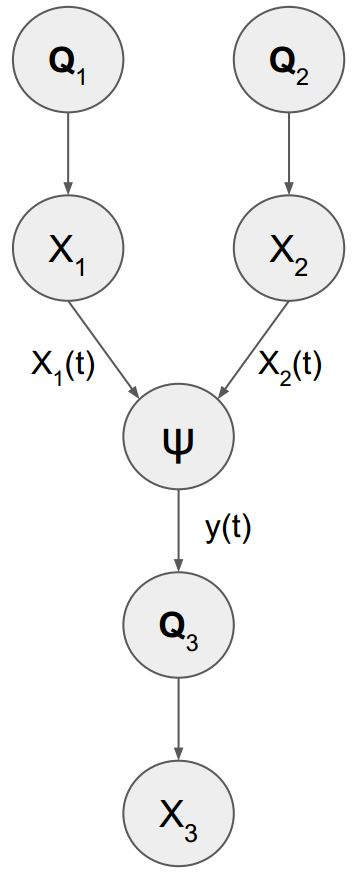
\includegraphics[width=0.6\linewidth]{figures/h_model}
	\caption{Hierarchical model.}
	\label{fig:h_model}
\end{wrapfigure} 
A detailed graphical model explored in this thesis is given in the \cref{fig:h_model}. This model presents an intersection of CTBN and POMDP frameworks. 
\begin{itemize}
	\item The transition models of the nodes $ X_1, X_2$ and $ X_3 $, and the dependencies between them are modelled as CTBN.
	\item The interaction of agent node $ X_3 $ and its environment is modelled as POMDP.
\end{itemize}

\subsection{CTBN Model}
\label{sec:exp_ctbn_model}
The transition models of the nodes and the dependencies between them are modelled as CTBN, denoted by S with graph $ \mathcal{G} = \left( \mathcal{V}, \mathcal{E}\right) $, where $ \mathcal{V} = \left\lbrace 1, 2, 3 \right\rbrace $ and $ \mathcal{E} = \left\lbrace (1, 3), (2, 3)\right\rbrace  $. The state of the nodes evolve as local variables $ X_n $, $ n\in \mathcal{V} $, and each variable has a state space denoted by $ \rchi_n $. The network S represents a stohastic process over a structured factorising state space $ \mathcal{S} = \rchi_1 \times \rchi_2 \times \rchi_3 $.\\
The parent nodes $X_{1}$ and $ X_{2} $ emit their states as messages. The dynamics  of these nodes are modelled as independent homogeneous continuous-time Markov processes $X_{n}(t)$, with binary-valued states $ \rchi_{n} = \left\lbrace 0, 1 \right\rbrace  $ for $ n \in \left\lbrace 1,2 \right\rbrace $. These processes are defined by transition intensity matrices $ \textbf{Q}_{n} $, which are assumed to be Gamma distributed with shape and rate parameters $ \symbf{\alpha} = [\alpha_0, \alpha_1] $ and $ \symbf{\beta} = [\beta_0, \beta_1] $, respectively, and are in the following forms.
\begin{align}
\textbf{Q}_n &= 
\begin{bmatrix}
-q^n_{0} & q^n_{0} \\
q^n_{1} &  -q^n_{1}
\end{bmatrix}
\label{eq:Q_parents}\\
\textbf{Q}_{n} &\sim \mathrm{Gam}(\symbf{\alpha}^n, \symbf{\beta}^n)\ \ \text{for}\ n \in \left\lbrace 1,2\right\rbrace \label{eq:gamma_priors}
\end{align}
It should be noted that in \autoref{eq:Q_parents}, the suffixes are simplified using the fact that $ q_{i} = \sum_{i \neq j} q_{i,j}$.\\
The agent  $ X_{3} $ is modelled as inhomogenouos continuous-time Markov process with binary states $ \rchi_{3} = \left\lbrace 0, 1 \right\rbrace  $, a set of actions $ a \in \left\lbrace a_0, a_1\right\rbrace  $, and a set of transition intensity matrices which contains one matrix corresponding to each action, $ \textbf{\textit{Q}}_{3 \mid a} = \left\lbrace \textbf{Q}_{3\mid a_{0}}, \textbf{Q}_{3\mid a_{1}} \right\rbrace $.\\
%\begin{equation}
%\textbf{Q}_{a_k} \sim \mathrm{Gam}(\alpha_{a_k}, \beta_{a_k})
%\end{equation}
The dependencies are represented by a set of parents for each node $ U_{n} = \mathrm{Par}_{\mathcal{G}}(X_n) $ and for the model shown in \cref{fig:h_model} can be written as follows:
\begin{align*}
U_{1}, U_{2} & = \emptyset \\
U_{3} & = \left\lbrace X_1, X_2 \right\rbrace 
\end{align*}
In order to have a compact representation of parent messages, a subsystem of S consisting of only the parent nodes $ X_1 $ and $ X_2 $ can be considered as a single system. These two processes can be represented as a \textit{joint} process, $ X_P $, with factorising state space $ \rchi_{P} = \rchi_1 \times \rchi_2  $. The transition intensity matrix of the new joint system, $ \textbf{Q}_P $ is obtained by amalgamation operation, denoted by *, between $ \textbf{Q}_{1} $ and  $ \textbf{Q}_{2} $ (see \cref{ap:amalgamation}) \cite{Nodelman1995}.
\begin{equation}
\textbf{Q}_P = \textbf{Q}_{1} * \textbf{Q}_{2}
\end{equation}

\subsection{POMDP Model}
\label{sec:exp_pomdp_model}
In a conventional POMDP scenario, there are two problems to be addressed, one is belief state update and the other is policy optimization. As mentioned in \cref{sec:belief_POMDP}, in the problem at hand, the policy of agent $ X_3 $ is assumed to be optimal and given. Thus, the POMDP model of the agent only consists of belief state update. A detailed view of the agents interaction with its environment from POMDP framework perspective is given in the \cref{fig:POMDP_pers}. \\
\begin{figure}[H]
	\begin{center}
		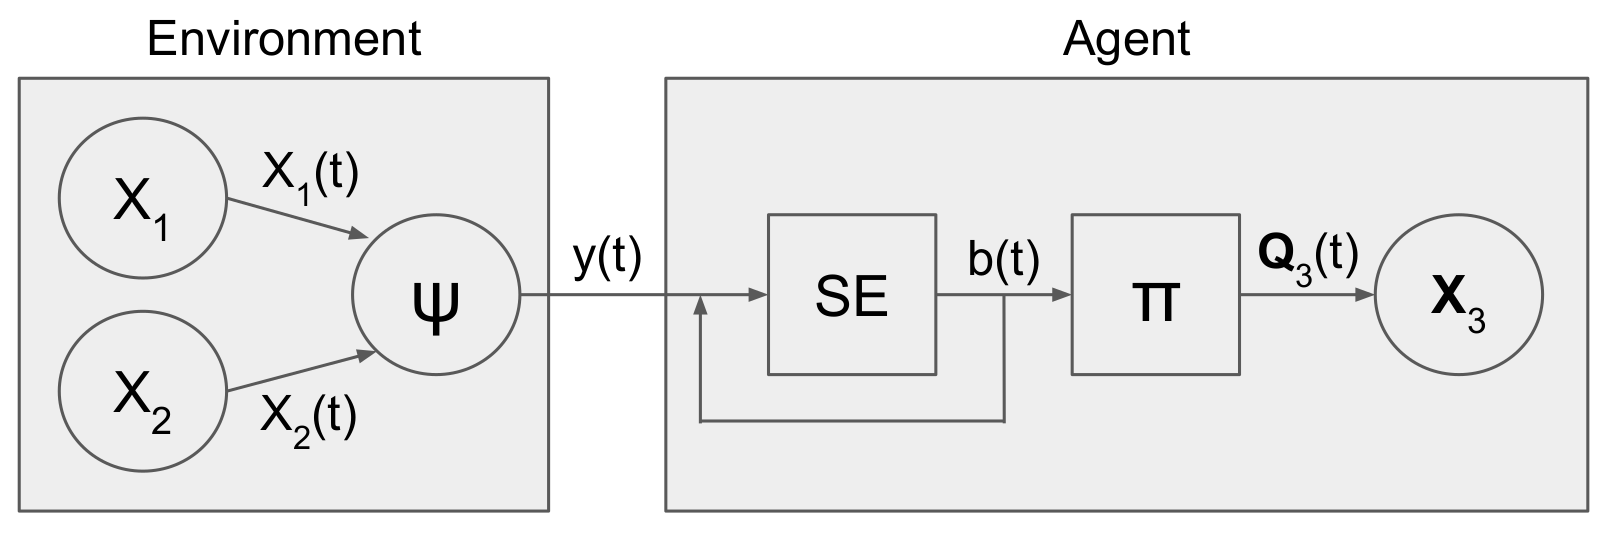
\includegraphics[width=.75\textwidth]{figures/POMDP_graph}
		\caption{A closer look at the agent-environment interaction from the perspective of POMDP framework.}
		\label{fig:POMDP_pers}
	\end{center}
\end{figure}
It should be noted that, the interaction in \cref{fig:POMDP_pers} is only one-sided, the state or action of the agent does not affect the environment.
\subsubsection{Observation Model}
\label{sec:observ_model}
The messages sent by the parent nodes are translated by the observation model. The agent node $ X_3 $ does not have a direct access to the messages, but observes a translation of them. The observation is denoted by $ y(t) = y_t $ such that $ y_t \in \mathcal{Y} $ where $ \mathcal{Y} $ is the observation space. The observation model defines a probability distribution over the observation for each combination of parent messages.
\begin{equation}
\psi(x_1, x_2) = p(y(t) \mid X_{1}(t)=x_1, X_{2}(t)=x_2)
\label{eq:obs_model_two_system}
\end{equation}
where $ x_1 \in \rchi_1 $ and $ x_2 \in \rchi_2 $. As explained in \cref{sec:exp_ctbn_model}, using the joint process $ X_P $ for the sake of conciseness, \autoref{eq:obs_model_two_system} can be written as
\begin{equation}
\psi(x_P) = p(y(t) \mid X_P(t)=x_P)
\label{eq:obs_model_p}
\end{equation}
where $ x_P \in \rchi_P $. \\
$ \psi(x_P) $ is defined as deterministic categorical distribution over the observation space $ \mathcal{Y} $. For each state $ x_P $, there is one possible observation $ y_i \in \mathcal{Y} $, such that \begin{equation}
p(y_i \mid x_P) = 1 \;\wedge \;p(y_j \mid x_P) = 0 \quad \forall j \neq i .
\label{eq:det_cat_dist}
\end{equation} 
$ \psi $ denotes the matrix with rows $ \left\lbrace \psi(x_P)\right\rbrace_{x_P \in \rchi_P} $.
\subsubsection{Belief State}
The belief state provides a summary over agent's past experiences and allows the agent to take its own uncertainty into account. The belief state is formed by the \textit{state estimator} (labelled as \textit{SE} in \cref{fig:POMDP_pers}) over the parent states, denoted by $  b(x_P; t) $. 
\begin{equation}
b(x_P; t) = \operatorname{Pr}( X_P(t) = x_P \mid y_{1}, ..., y_{t})
\end{equation}
The initial belief state is assumed to be uniformly distributed, and is updated with the first observation at $ t_0 = 0 $.
\paragraph*{Exact Belief State Update}
\label{par:bs_exact}
As discussed in \cref{sec:filtering_CTMC}, given the transition intensity matrices of parent nodes, $ \textbf{Q}_1 $ and $ \textbf{Q}_2 $, the continuous-time belief state update poses a filtering problem for CTMPs. This problem can be formulated according to the joint process of parents.
\begin{equation}
b(x_P; t) = \operatorname{Pr}( X_P(t) = x_{p} \mid y_{1}, ..., y_{t})
\end{equation}
Consider discrete-time observations from this process, denoted by $ y_{1}=y(t_{1}), ..., y_{l}=y(t_{l}) $ and time-dependent belief state $ b(t) $ as a row vector with $ \left\lbrace b(x_P;t)\right\rbrace_{x_P \in \rchi_P} $. Following \autoref{eq:b_cont} and \autoref{eq:b_jump}, the belief state update is evaluated as
\begin{equation}
b(t) = b(0) \exp(t\textbf{Q}_P)
\end{equation}
with the initial condition $ b(0) $.
The update at discrete times of observation $ y_{t} $ is
\begin{align}
b(x_P; t_{l}) &= Z_{l}^{-1}\ {p(y_{l} \mid X_P(t_{l})=x_P)}\ {b(x_P; t_{l}^{-})} \\ & = Z_{l}^{-1}\ \psi(x_P) \ {b(x_P; t_{l}^{-})}
\label{eq:bs_exact}
\end{align}
where $ Z_{l} = \sum_{x_P\in \rchi_P} \psi(x_P)\ b(x_P; t_{l}^{-}) $ is the normalization factor.
\paragraph*{Belief State Update Using Marginalized Particle Filter}
\label{par:bs_partFilt}
The assumption that the complete information of parent dynamics is available is unrealistic. In an environment as described above, the agent is more likely not to have access to the parameters $ \textbf{Q}_1 $ and $ \textbf{Q}_2 $. It may rather have some prior beliefs over them. Moreover, when the state estimator utilizes exact update method, these parameters are assumed to be available for the inference as well. Thus, in order to simulate a more realistic model and be able to marginalize out these parameters from inference problem, the joint parent process $ X_P $ is replaced with its marginalized counterpart. Using the Gamma-priors over $ \textbf{Q}_1 $ and $ \textbf{Q}_2 $ (\autoref{eq:gamma_priors}) and sufficient statistics over the particle history, the particles are drawn from this marginalized process as explained in \cref{sec:marg_ctbn}. With every new observation, the particles are propogated through the marginal process. The processing of the particles are done one after another as explained in \cref{sec:marg_ctbn}. After propagating each particle, the summary statistics are updated and the parameters are re-estimated using the \autoref{eq:estimated_Q}. The belief state is then obtained as the distribution of states over the particles,
\begin{equation}
b(x_P; t) = \frac{1}{M} \sum_{m=1}^{M} \delta_{k_m(t), x_P}
\label{eq:belief_over_particles}
\end{equation}
where $ M $ is the number of particles, $ k_i \in \textbf{k} $ is the set of particles, and $\delta$ is the Kronecker delta.

\begin{algorithm}[H]
	\SetKwInOut{KwIn}{Input}
	\SetKwInOut{KwOut}{Output}
	\KwIn{Observation $ y_{l} $ at time $ t_{l} $, set of particles $\textbf{k}^{l-1} $, estimated $ \hat{Q} $}
	\KwOut{New set of particles $ \textbf{k}^{l} $, $ \textbf{b}^{[t_{l-1}, t_{l}]} $}
	
	\vspace{+4pt}
	\begin{algorithmic}[1]
		\FOR{$k_{m} \in \textbf{k}^{l-1}$}
		\STATE {$k_{m} = \left\lbrace x_{m}, \hat{Q}\right\rbrace \leftarrow Propagate\ particle\ through\ marginal\ process\ from\ t_{l-1}\ to\ t_{l}$ }\\
		
		\STATE {$\hat{Q} \leftarrow sufficient\ statistics\ added\ from\  k_{m}[t_{l-1}, t_{l}]$} \\
		\tcp*[h] {observation likelihood assigned as particle weight}
		\STATE{$w_{m} \leftarrow p(y_{l} \mid X_P(t_{l})=x_{m}) $} \label{lst:weight_update}
		\ENDFOR \\
		\tcp*[h]{belief state from $ t_{l-1} $ to $ t_{l} $}
		\STATE{$ \textbf{b}^{[t_{l-1}, t_{l}]} \leftarrow \left\lbrace \frac{1}{M} \sum_{m=1}^{M} \delta_{k_m^{[t_{l-1}, t_{l}]} , x_P}\right\rbrace_{x_P \in \rchi_P} $}\\
		\tcp*[h]{normalize weights}
		\STATE{$ w_{m} \leftarrow \frac{w_{m}}{\sum_{m} w_{m}}$   }\\
		\tcp*[h]{  resample particles}
		\FOR{$ k_{m} \in \textbf{k}^{l} $} 
		\STATE{$ k_{m} \leftarrow Sample\ from\ \textbf{k}^{l}\ with\ probabilities\ w_{m}\ with\ replacement$}
		\ENDFOR 
	\end{algorithmic}
	\caption{Marginal particle filter for belief state update \cite{Studer2016}}
	\label{alg:part_filter}
\end{algorithm}
In \cref{alg:part_filter}, the weight update for the particles is performed on line \autoref{lst:weight_update}, based on the observation model. Given the deterministic nature of the observation model as described in \autoref{eq:det_cat_dist}, in rare cases where the observation $ y_k $ stems from an unlikely transition of parent nodes, the particles fail to simulate this transition and all of them are rejected. One possible solution to this problem would be to increase the number of particle to increase the probability of sampling unlikely transitions. However, in practice, this solution is computationally infeasible. Instead, the degeneration of the particle filter is dealt with by assigning uniform probabilities to the particles, effectively ignoring the unlikely transitions. The situation is illustrated by examples from simulation in \cref{sec:simulation}.

\subsubsection{Optimal Policy}
The optimal policy is defined using a polynomial function of belief state.
\begin{equation}
\pi(b) = 
\begin{cases}
a_0 & \quad \text{if } \textbf{w}b^\intercal > 0.5 \\
a_1 & \quad \text{otherwise}
\end{cases}
\label{eq:policy}
\end{equation}
where \textbf{w} is a row vector of weights.\\
Given the optimal policy, $ \pi(b) $, the agent takes an action based on the belief state. In the setting described above, taking an action means to change its internal dynamics to the transition intensity matrix corresponding to that action.
\begin{align}
a(t) &= \pi(b(t))\\
\textbf{Q}_3(t) & = \begin{cases}
\textbf{Q}_{3\mid a_{0}} & \quad \text{if } a(t) = a_0 \\
\textbf{Q}_{3\mid a_{1}} & \quad \text{otherwise}
\end{cases}
\label{eq:Q_3_traj}
\end{align}

\section{Inference of Observation Model}
\label{sec:inf_setup}
Inference problem is considered for deterministic observation models, such that each state $ x_P \in \rchi_P $ can only be translated to one observation. Considering the number of states of parents and the observations, this results in a number of possible observation models. \\
Consider a trajectory in the dataset, denoted by $ S^{[0,T]} = \left\lbrace X_1^{[0,T]} , X_2^{[0,T]}, X_3^{[0,T]}\right\rbrace $. The set of parameters to the system, as introduced before, is written as $  \theta = \left\lbrace  \textbf{Q}_{1}, \textbf{Q}_{2}, \textit{\textbf{Q}}_3, \pi, \psi \right\rbrace $. Given the parent trajectories, $ X_1^{[0,T]} $ and $ X_2^{[0,T]} $, the belief state and the resulting $ \textbf{Q}_3 $ trajectory are computed for each observation model. Then the likelihood of $ S^{[0,T]} $ trajectory given the parameters $ \theta $ are used for classifiation task.

\subsection{Likelihood Model}
 The likelihood of a sample trajectory $ S^{[0,T]} $ can be written as:
\begin{align}
p(S^{[0,T]} \mid \theta ) & = p(X_{1}^{[0, T]}, X_{2}^{[0, T]}, X_{3}^{[0, T]} \mid \textbf{Q}_{1}, \textbf{Q}_{2}, \textit{\textbf{Q}}_3, \pi, \psi) \nonumber\\
& = p(X_{3}^{[0, T]} \mid X_{1}^{[0, T]}, X_{2}^{[0, T]}, \textbf{Q}_{1}, \textbf{Q}_{2}, \textit{\textbf{Q}}_3, \pi, \psi) \ p(X_{1}^{[0, T]}\mid \textbf{Q}_{1}) \ p(X_{2}^{[0, T]}\mid \textbf{Q}_{2}) \nonumber\\ & = p(X_{3}^{[0, T]} \mid X_{1}^{[0, T]}, X_{2}^{[0, T]}, \textit{\textbf{Q}}_3, \pi, \psi) \ p(X_{1}^{[0, T]}\mid \textbf{Q}_{1}) \ p(X_{2}^{[0, T]}\mid \textbf{Q}_{2}) \nonumber\\ & = p(X_{3}^{[0, T]}\mid \textbf{Q}_{3}^{[0, T]}) \ p(X_{1}^{[0, T]}\mid \textbf{Q}_{1}) \ p(X_{2}^{[0, T]}\mid \textbf{Q}_{2}) 
\label{eq:system_llh}
\end{align}
As mentioned before, it is plausible to marginalize out the parameters $ \textbf{Q}_1 $ and $ \textbf{Q}_2 $, for a more realistic model and inference. Noting that in case the belief state is updated using by filtering CTMPs (See \cref{par:bs_exact}), $ \textbf{Q}_{3}^{[0, T]} $ becomes a deterministic function of all the parameters including $ \textbf{Q}_1 $ and $ \textbf{Q}_2 $, the marginalization cannot be carried out analytically on \autoref{eq:system_llh}. On the other hand, marginal particle filtering removes this dependency on $ \textbf{Q}_1 $ and $ \textbf{Q}_2 $ by using marginalized counterpart of CTMPs (See \cref{par:bs_partFilt}), leaving it straightforward to marginalize out the parameters on \autoref{eq:system_llh}.

Marginalizing the likelihood over $ Q_{1} $ and $ Q_{2} $:
\begin{align}
p(S^{[0,T]} \mid \pi, \psi ) & = 	\int \int p(S^{[0,T]} \mid \theta ) \ p(\textbf{Q}_{1}) \ p(\textbf{Q}_{2}) \ d\textbf{Q}_{1}d\textbf{Q}_{2} \nonumber\\ 
& = \int \int p(X_{3}^{[0, T]}\mid \textbf{Q}_{3}^{[0, T]}) \ p(X_{1}^{[0, T]}\mid \textbf{Q}_{1}) \ p(X_{2}^{[0, T]}\mid \textbf{Q}_{2}) \ p(\textbf{Q}_{1}) \ p(\textbf{Q}_{2})\ d\textbf{Q}_{1}d\textbf{Q}_{2} \nonumber\\ 
& = p(X_{3}^{[0, T]}\mid \textbf{Q}_{3}^{[0, T]}) \int  p(X_{1}^{[0, T]}\mid \textbf{Q}_{1}) \ p(\textbf{Q}_{1}) \ d\textbf{Q}_{1} \int p(X_{2}^{[0, T]}\mid \textbf{Q}_{2})\ p(\textbf{Q}_{2})\ d\textbf{Q}_{2}
\label{eq:Marg_llh}
\end{align}
Marginalized likelihood function for binary-valued homogenous CTMP is derived in \autoref{ap:marg_llh_ctmp}.

Plugging \autoref{eq:Marg_traj} in \autoref{eq:Marg_llh} for both $ X_{1} $ and $ X_{2} $:
\begin{align}
\begin{split}
p(S^{[0,T]} \mid \pi, \Phi ) = p(X_{3}^{[0, T]}\mid Q_{3}^{[0, T]}) \prod_{x_{1}\in{0,1}} \frac{\beta_{x_{1}}^{\alpha_{x_{1}}}}{\Gamma(\alpha_{x_{1}})} \ (\Upsilon(x_{1})+\beta_{x_{1}})^{r(x_{1}) + \alpha_{x_{1}}}\ \Gamma(r(x_{1}) + \alpha_{x_{1}})  \\  \prod_{x_{2}\in{0,1}} \frac{\beta_{x_{2}}^{\alpha_{x_{2}}}}{\Gamma(\alpha_{x_{2}})} \ (\Upsilon(x_{2})+\beta_{x_{2}})^{{r(x_2)} + \alpha_{x_{2}}}\ \Gamma(r(x_2) + \alpha_{x_{2}})
\label{eq:Marg_llh_final}
\end{split}
\end{align}

\subsection{Inference under Noisy Observation Model}
\label{sec:noisy_robustness}
In order to assess the robustness of the inference, we added an error probability $ p_e $ to the observation model. As explained in \cref{sec:observ_model}, the observation model $ \psi(x_P) $ is assumed to be deterministic. This corresponds to a unique translation, denoted here by $ y_\text{true} $, of each parent state $ x_P $. In the case of noisy observation model, the resulting observation might differ from the correct translation $ y_\text{true} $ with probability $ p_e $, and the erroneous translation is drawn uniformly from the remaining observation space $ y_i \in \mathcal{Y} \backslash \left\lbrace y_\text{true}\right\rbrace $. This noisy observation model, denoted by $ \psi^{p_e} $, can be considered as a noisy communication channel with error probability $ p_e $. \begin{equation}
p(y_\text{true} \mid x_P) = 1-p_e \;\wedge \;p(y_j \mid x_P) = \frac{p_e}{|\mathcal{Y}|-1} \quad \forall y_j \neq y_\text{true}
\label{eq:noicy_obs_model}
\end{equation} 
For simulation, the noisy observation model is assumed to be available to the agent, which mainly affects the agent's belief state. For exact belief state update, the noisy observation model is employed in \autoref{eq:bs_exact}. In the case of particle filtering, the weights are assigned to the particle using the noisy model (see \cref{alg:part_filter}, line \autoref{lst:weight_update}). It is noteworthy that by doing so, the degeneration of particle filter as described in \cref{par:bs_partFilt} is prevented.
\subsection{Performance Metrics}
As a measure of the performance of the classifier, we utilised area under the Reciever-Operator-Characteristic curve (AUROC) and Precision-Recall curve (AUPR). Since our setting presents a multi-class classification problem, the
performance metrics AUROC and AUPR are evaluated as one-vs-rest.\\
Consider a binary classification problem with class labels 0 and 1. True positives (TP) are the samples predicted as 1 correctly, and false positives (FP) are the samples predicted as 1 while the true label was 0. True negatives (TN) are the samples predicted as 0 correctly, and false negatives (FN) are the samples with true label 1, but predicted 0. True positive rate (TPR), also called \textit{recall} (R) or \textit{sensitivity}, is the ratio of TPs over the number of samples which are labelled as 1. False positive rate (FPR) is the ratio of FPs over the number of samples labelled as 0. The precision (P) is the ratio of TPs over the number of all the samples predicted as 1.
\begin{align}
\text{TPR} = \text{R} &= \frac{\text{TP}}{\text{TP} + \text{FN}} \\
\text{FPR} &= \frac{\text{FP}}{\text{TN} + \text{FP}} \\
\text{P} &= \frac{\text{TP}}{\text{TP} + \text{FP}}
\end{align}
Receiver Operating Characteristics (ROC) curve illustrates the tradeoff between true positives and false positives, over different values of threshold for classification \cite{kerekes2008receiver}. The area under ROC curve is a performance metric that shows how well the classifier can distinguish the classes. Higher AUROC metric indicates better performance, taking values in the interval [0,1]. Precision-Recall (PR) curve illustrates the relation between precision and recall, providing a metric to quantify how many of the predictions were correct \cite{Boyd2013}.
\section{Data Generation}
The dataset contains a number of trajectories drawn from CTBN $ S $. Following the notation in \cref{chap:2}, $ K $ trajectories in time interval $ [0, T] $ are denoted by $ \xi_T = \left\lbrace S^{[0,T], 1}, S^{[0,T], 2}, ..., S^{[0,T], K} \right\rbrace  $, where $ S^{[0,T],\kappa} = \left\lbrace X_1^{[0,T],\kappa} , X_2^{[0,T],\kappa}, X_3^{[0,T],\kappa}\right\rbrace $ denotes a single trajectory for all nodes. Every trajectory comprises of state transitions in the interval, and the times of these transitions. 
\subsection{Sampling Algorithm}
In order to sample trajectories from CTBN, two sampling algortihms introduced in \cref{sec:sampling_alg} are combined. Gillespie algorithm is used to sample from the parent nodes, $ X_1 $ and $ X_2 $, while thinning algorithm is applied to overcome the challenges that come with conditional intensity matrix of the agent, $ X_3 $. It should be noted that \cref{alg:generative_ctbn} is applicable to any nodes in a CTBN, both homogenous and conditional MPs. However, since in this setting, the intensity matrix is conditioned on the belief state and the policy, instead of directly on the parent states, a more general algorithm suitable for inhomogenous MPs, thinning algorithm, is preferred. \cref{alg:sampling} describes the procedure to draw samples using marginal particle filtering. \\
\begin{algorithm}[H]
	\SetKwInOut{KwIn}{Input}
	\SetKwInOut{KwOut}{Output}
	\SetKwInOut{Init}{Initialize}
	
	\KwIn{Gamma-prior parameters on parents' transition intensity matrices $ \alpha^1, \beta^1, \alpha^2, \beta^2 $\\
		Set of agent's transition intensity matrices $ \textbf{\textit{Q}}_3 $\\
		$ T_{max} $ to terminate simulation}
	\KwOut{Sample trajectory of the network}
	\Init{Sample $ \textbf{Q}_1 $ and $ \textbf{Q}_2 $ from their priors\\ 
		Initialize nodes uniformly $ X_{n}(0) = x_{n} \in \rchi_n$ \\
		Initialize particles uniformly $ k^i(0) = x_{p} \in \rchi_P$\\
		$ t=0 $}
	
	\begin{algorithmic}[1]
		\WHILE{$ t < T_{max} $}
		\STATE{Draw next transition for $ X_1 $ and $ X_2 $ ($ \tau_{parent}$, $ x_1 $ and $ x_2 $ using \cref{alg:generative_ctbn})}
		\STATE{$ t_{parent} \leftarrow t + \tau_{parent} $}	\tcp*[h]{transition time for parents} 
		\STATE{$ y_{t_{parent}} \sim \psi(x_1, x_2)$} \tcp*[h]{new observation at $ t_{parent} $}
		\STATE{Update particle filter and obtain $ \textbf{b}^{[t, t_{parent}]} $}
		\STATE{$ a^{[t, t_{parent}]} \leftarrow \pi(\textbf{b}^{[t, t_{parent}]}) $}
		\STATE{$ \textbf{Q}_3^{[t, t_{parent}]} \leftarrow \textbf{Q}_{3\mid a^{[t, t_{parent}]}} $}
		\STATE{$ t_{agent} \leftarrow t$}
		\WHILE{$ t_{agent} < t_{parent} $}
		\STATE{\text{the upper bound for intensity,} $ q_3^{*}$} \footnotemark
		\STATE{\text{transition time $ \tau_{agent} $ drawn by }  $ u \sim U(0, 1)$ \text{ and } $ \tau_{agent} = \frac{-ln(u)}{q_3^{*}} $}
		\STATE{$ t_{agent} \leftarrow t_{agent} + \tau_{agent} $}
		\STATE{\text{draw } $s \sim U(0, 1)$, \text{accept transition if} $ s \leq \frac{q_3(t_{agent})}{q_3^{*}}$}
		\ENDWHILE
		\STATE{$ t \leftarrow t_{parent} $}
		\ENDWHILE
	\end{algorithmic}
	\caption{Sampling trajectories with marginal particle filtering}
	\label{alg:sampling}
\end{algorithm}
\footnotetext{q is the transition intensity associated with the current state of the agent.}

%\begin{table}[!htb]
%	\begin{minipage}{.5\linewidth}
%		%		\centering
%		\begin{tabular}{c c}
%			\hline 
%			\textbf{Parameter} & \textbf{Value} \\ 
%			\hline 

%			\hline 
%		\end{tabular}
%		\caption{configuration}
%	\end{minipage}%
%	\begin{minipage}{.5\linewidth}
%		%		\centering
%		\begin{tabular}{c c c}
%			\hline 
%			\textbf{Parameter} & \textbf{Value} 
%			\hline 

%			\hline 
%		\end{tabular}
%		\caption{configurations}
%	\end{minipage} 
%\end{table}

	%\externaldocument[-f]{c2_foundations}
%\externaldocument[-f]{c3_simulation_experiments}
\chapter{Results}
\label{chap:4}
The experimental results are presented in this chapter. First, the parameters for the variables introduced in \cref{chap:3} are given. Then a sample of simulated trajectories are shown as an example. Finally, the inference results are presented.

\section{Configurations}
\label{sec:config}
The configurations given below are used for the results presented in the following sections, if not specified otherwise.
\begin{itemize}
	\item Gamma priors for parent dynamics such that $ \textbf{Q}_{i} \sim \mathrm{Gam}(\symbf{\alpha}^i, \symbf{\beta}^i)$ for $i \in \left\lbrace 1,2\right\rbrace $, and $ \symbf{\alpha} = [\alpha_0, \alpha_1] $ and $ \symbf{\beta} = [\beta_0, \beta_1] $
	\begin{align}
	\symbf{\alpha}^1 = [5,10] &\quad \symbf{\beta}^1 = [5,20] \\
	\symbf{\alpha}^2 = [10,10] &\quad \symbf{\beta}^2 = [10,5]
	\label{eq:gamma_params}
	\end{align}
	\item Transition intensity matrices of $ X_1 $ and $ X_2 $ sampled from priors given above
	\begin{align}
	\textbf{Q}_1 &= 
	\begin{bmatrix}
	-1.117 & 1.117 \\
	0.836 &  -0.836
	\end{bmatrix} \\
	\textbf{Q}_2 &= 
	\begin{bmatrix}
	-1.1 & 1.1 \\
	2.445 &  -2.445
	\end{bmatrix}
	\end{align}
	\item Length of trajectories $ T = 5\text{s} $
	\item State space, $ \rchi_{P} = \rchi_1 \times \rchi_2 = \left\lbrace (x_1, x_2)\right\rbrace_{x_1\in \rchi_1, x_2\in \rchi_2} = \left\lbrace (0, 0), (0, 1), (1, 0),(1, 1)\right\rbrace $
	\item Observation space, $ \mathcal{Y} = \left\lbrace 0, 1, 2 \right\rbrace $
	\item Action space, $ \textit{A} = \left\lbrace a_{0}, a_{1} \right\rbrace = \left\lbrace 0, 1\right\rbrace $
	\item The set of transition intensity matrices of $ X_3 $
	\begin{align}
	\textbf{\textit{Q}}_3 = \left\lbrace \textbf{Q}_{3\mid a_{0}}, \textbf{Q}_{3\mid a_{1}} \right\rbrace = \left\lbrace 
	\begin{bmatrix}
	-0.5 & 0.5 \\
	2 &  -2
	\end{bmatrix}, 
	\begin{bmatrix}
	-3 & 3 \\
	0.02 &  -0.02
	\end{bmatrix} 
	\right\rbrace 
	\end{align}
	\item Number of particles, $ N = 200 $
	\item Weights of the policy introduced in \autoref{eq:policy}, $ \textbf{w} = [0.02, 0.833, 0.778, 0.87] $
	\item Observation model
	$\psi_{\text{true}} =
	\begin{bmatrix}
		1 & 0 & 0 \\
		0 & 1 & 0 \\
		0 & 1 & 0 \\
		0 & 0 & 1
	\end{bmatrix}$
%	\item Simulation parameters $  \theta_sim = \left\lbrace  \textbf{Q}_{1}, \textbf{Q}_{2}, \textit{\textbf{Q}}_3, \textbf{w}, \psi_{\text{true}} \right\rbrace $
\end{itemize}
%In the following, $ \psi_{\text{true}} $ denotes the observation model which is used for data generation in the given results.

\section{Simulation}
\label{sec:simulation}
The synthetic dataset is generated utilising \cref{alg:sampling}. K trajectories in time interval $ [0, T] $ are denoted by $ \xi_T = \left\lbrace S^{[0,T], 1}, S^{[0,T], 2}, ..., S^{[0,T], K} \right\rbrace  $, where $ S^{[0,T],k} = \left\lbrace X_1^{[0,T],k} , X_2^{[0,T],k}, X_3^{[0,T],k}\right\rbrace $ denotes a single trajectory for all nodes. It is noteworthy that the initial states are drawn from disrete uniform distribution.
\begin{equation}
X_i(0) \sim \mathcal{U} \left\lbrace 0, 1\right\rbrace  \text{ for } i \in \left\lbrace 1,2,3\right\rbrace 
\end{equation}
\autoref{fig:parent_traj}(a)-(b) shows an example of parent trajectories. In \autoref{fig:parent_traj}(c), the resulting trajectory of the joint parent process $ X_P $ is illustrated. As mentioned in \cref{sec:exp_ctbn_model}, this joint process over the parent nodes provides a compact representation. 
\begin{figure}[H]
	\begin{center}
		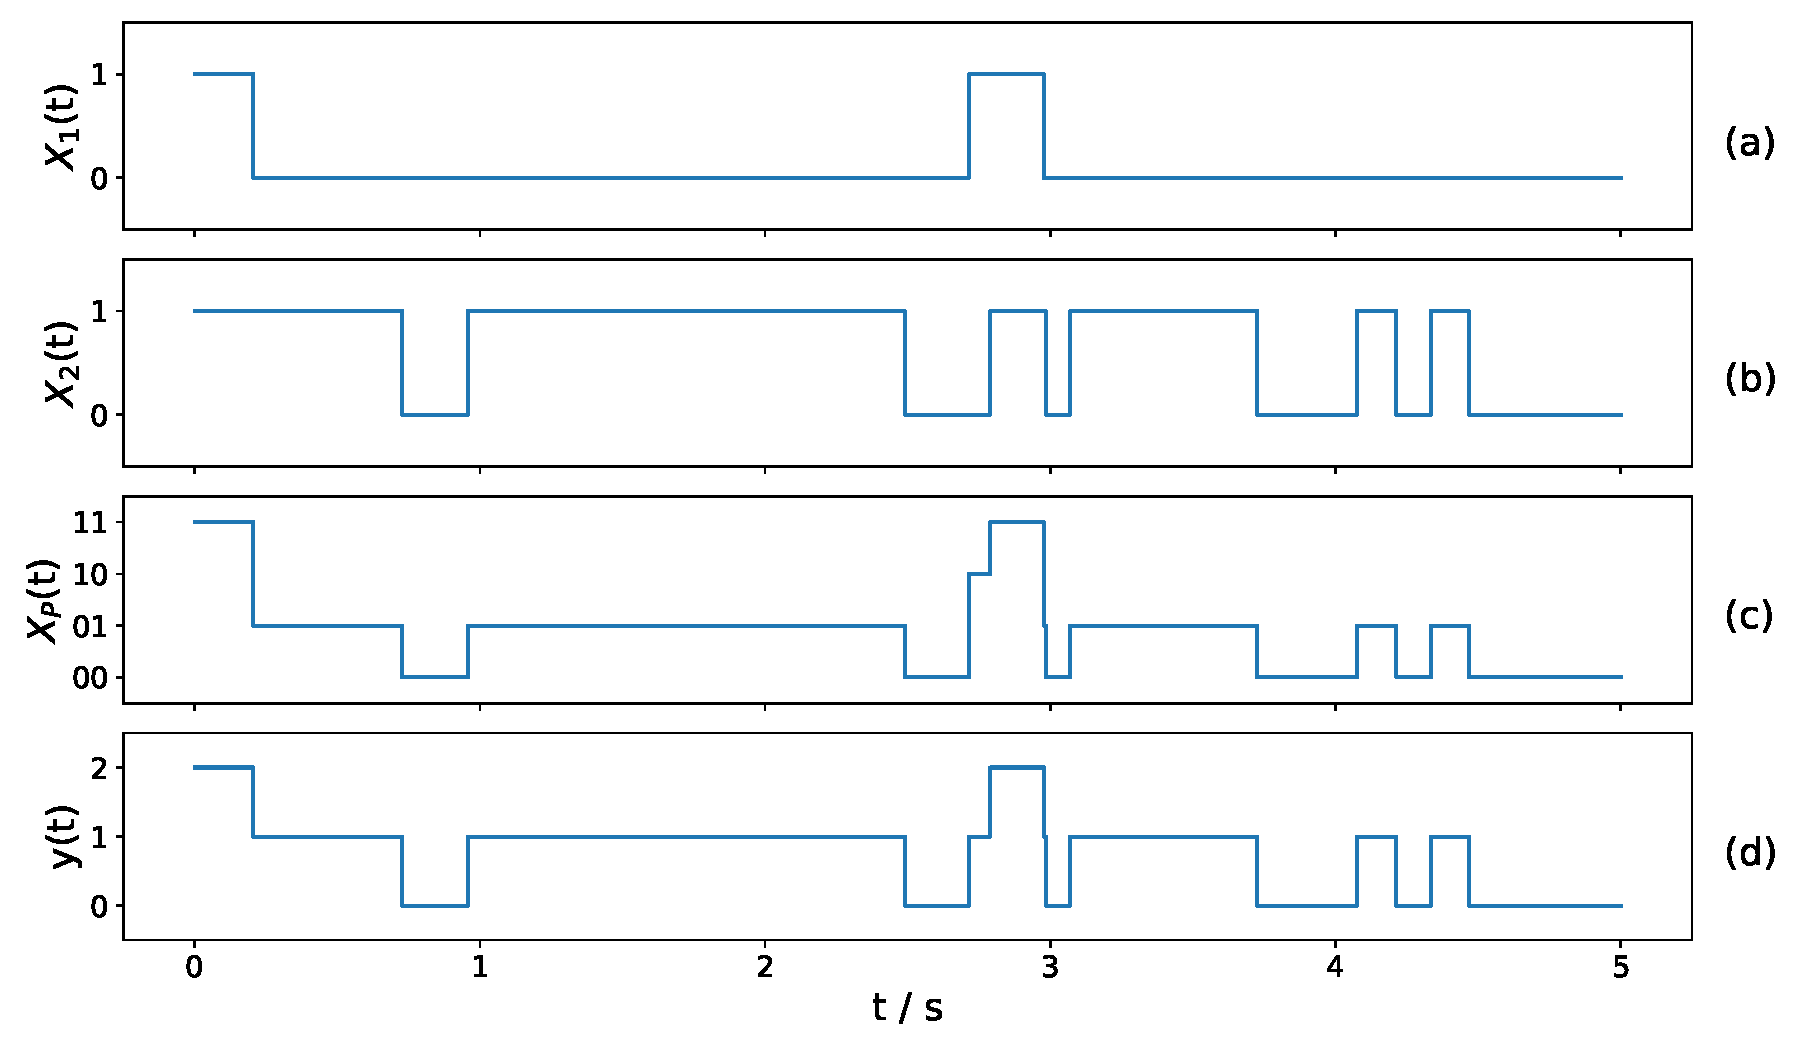
\includegraphics[width=.90\textwidth]{figures/sim_example/parent_traj}
		\caption[Parent trajectories and observation]{A sample of parent trajectories and observation. (a)-(b) A sample trajectory of parent nodes $ X_1 $ and $ X_2 $ of length $ T=5\text{s} $, (c) The trajectory of the joint parent process $ X_P $, (d) The observation trajectory resulting from $ X_P $ given in (c) and $ \psi_{\text{true}} $ given in \cref{sec:config}.}
		\label{fig:parent_traj}
	\end{center}
\end{figure}
In \autoref{fig:parent_traj}(c), the states of $ X_P $ taking values in $ \rchi_P = \rchi_1 \times \rchi_2 $ is preferred to be represented as a combination of the parent states for readibility, so that $ \rchi_P = \left\lbrace 00, 01, 10, 11\right\rbrace  $, where $ x_P \in \rchi_P $ simply corresponds to $ x_1x_2,\ x_1\in \rchi_1,\  x_2\in \rchi_2 $. \autoref{fig:parent_traj}(d) shows the observation trajectory resulting from $ X_P(t) $ and the observation model $ \psi_{true} $ given in \cref{sec:config}. \\
\autoref{fig:belief_traj} illustrates the belief state trajectory given the observations in \autoref{fig:parent_traj}(d). For the reference, the belief state update using marginal particle filter and exact update is given together. As can be seen from the figures, the exact update is well approximated by the particle filter.
\begin{figure}[H]
	\begin{center}
		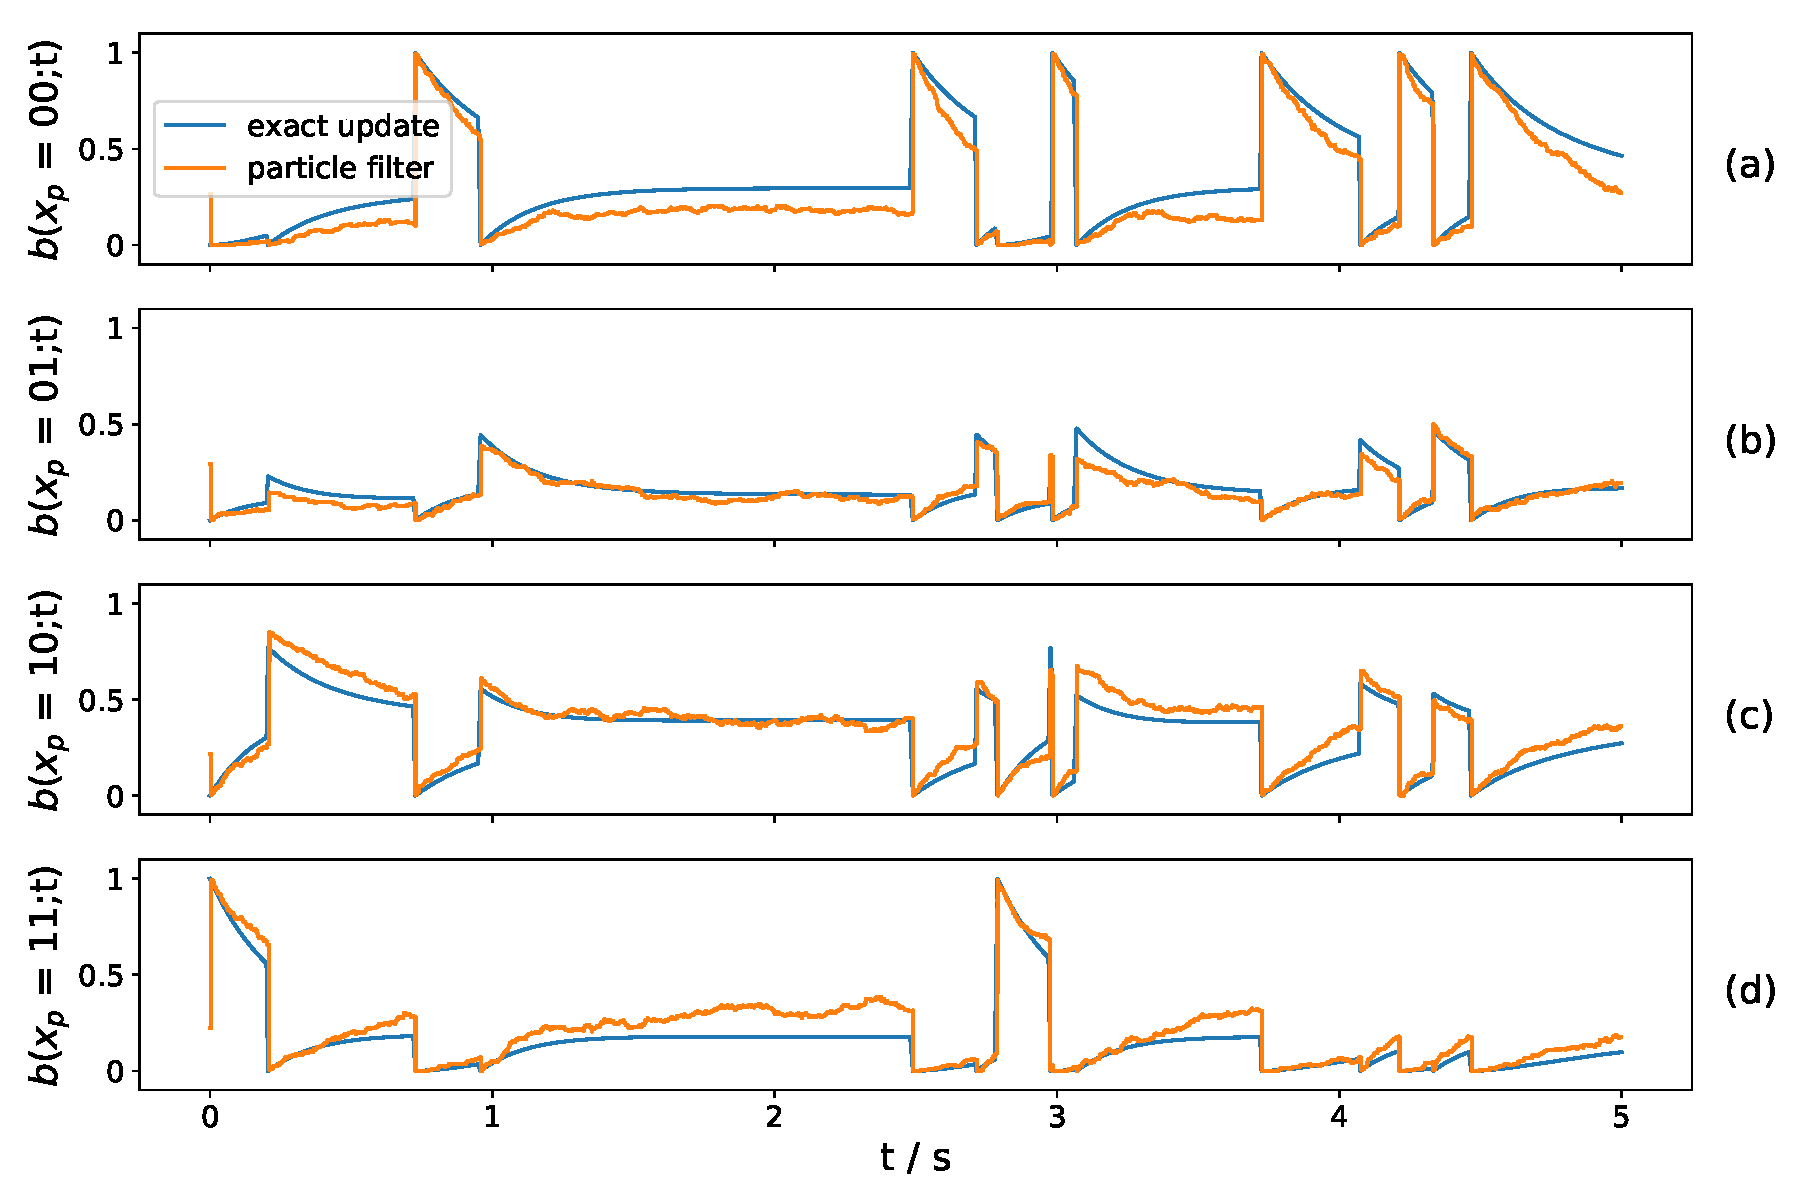
\includegraphics[width=.9\textwidth]{figures/sim_example/belief_traj}
		\caption[Belief state trajectories]{Belief state trajectories corresponding to the observations given in \autoref{fig:parent_traj}(d), comparing exact update method and marginal particle filtering.}
		\label{fig:belief_traj}
	\end{center}
\end{figure}
Finally, the resulting $ Q_3 $ and the trajectory of agent are given in \autoref{fig:q_traj}. The $ Q_3 $ trajectory shown in \autoref{fig:q_traj}(b), are derived from the belief state update by marginal particle filter which is given in \autoref{fig:q_traj}(a) using \autoref{eq:policy} and \autoref{eq:Q_3_traj}.
\begin{figure}[H]
	\begin{center}
		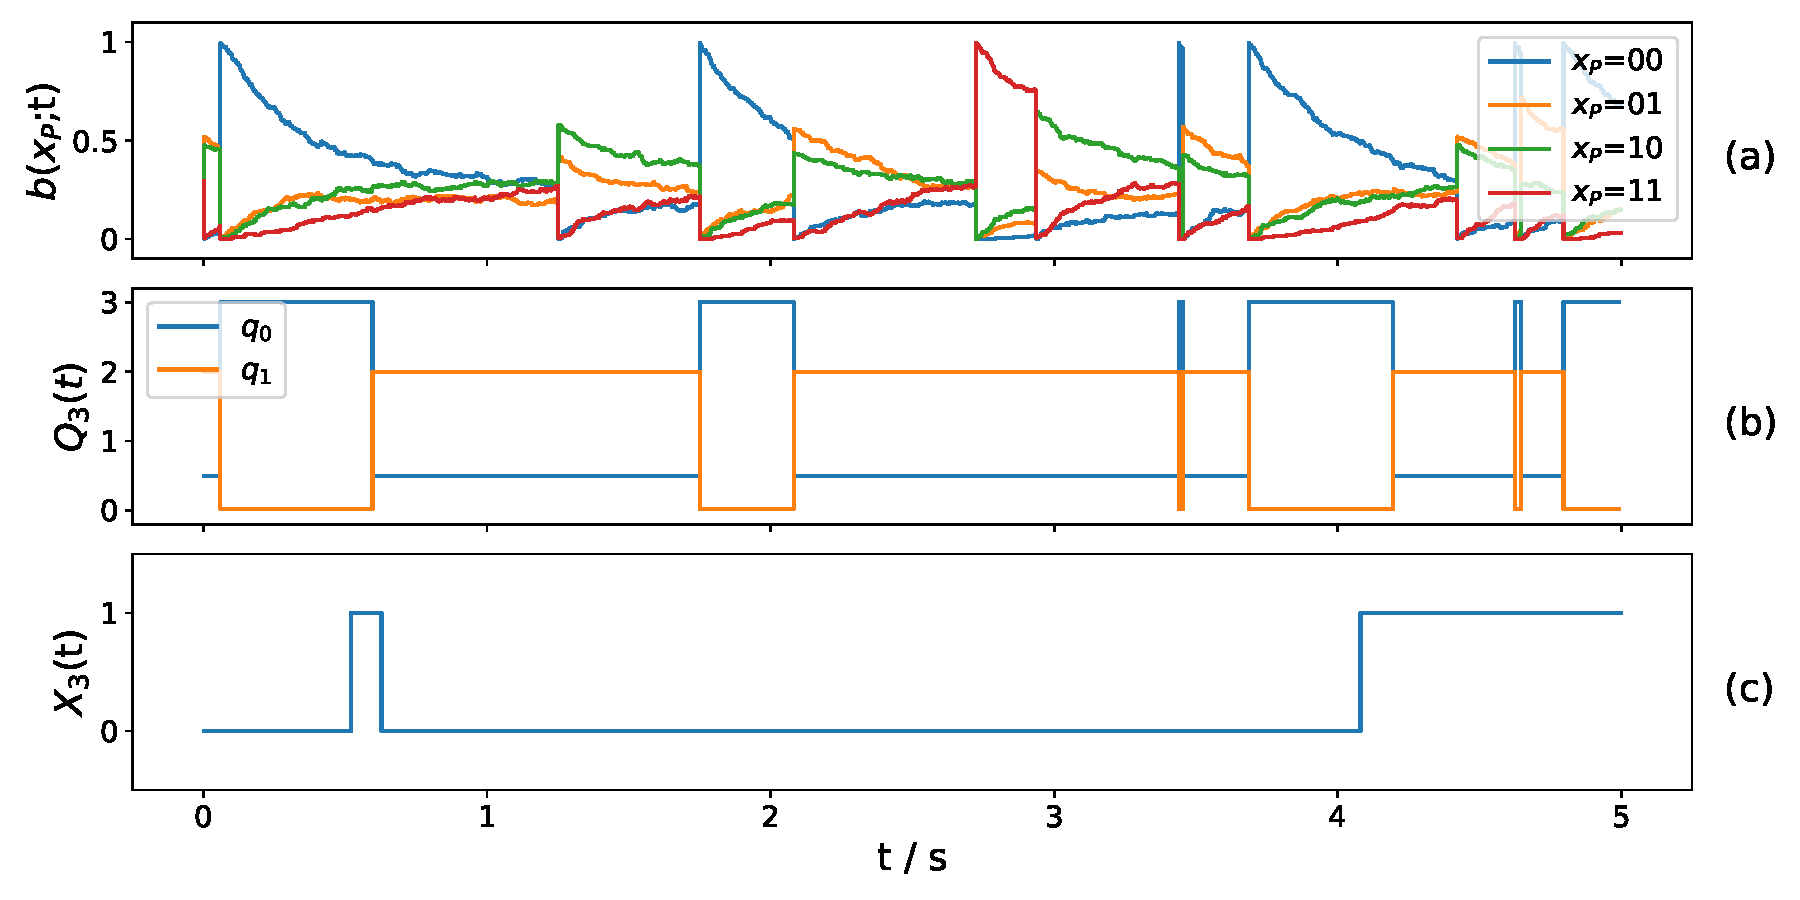
\includegraphics[width=.87\textwidth]{figures/sim_example/q_traj}
		\caption[$ Q_3 $ and $ X_3 $ trajectories]{Belief state updated by marginal particle filter and the resulting $ Q_3 $ and $ X_3 $ trajectories.}
		\label{fig:q_traj}
	\end{center}
\end{figure}
As mentioned in \cref{par:bs_partFilt}, the degeneration of the particle filter in case of an unlikely changes in observation, i.e. unanticipated transitions of parent nodes, is handled by by assigning uniform probabilities to the particles. It effectively corresponds to ignoring the rapid changes of the observation, which may cause diverging from the exact update, however, it is recovered with the next observation. \autoref{fig:deg_partFilter} provides an example of the sitution. The rapid change in question that caused particle filter method to diverge from exact update method is highlighted in \autoref{fig:deg_partFilter}(a). The particles fail to simulate this observation, and due to uniformization, the transition from 2 to 1 is ignored by the marginal particle filter method. The divergence can be observed in \autoref{fig:deg_partFilter}(d)-(e) clearly.
\begin{figure}[H]
	\begin{center}
		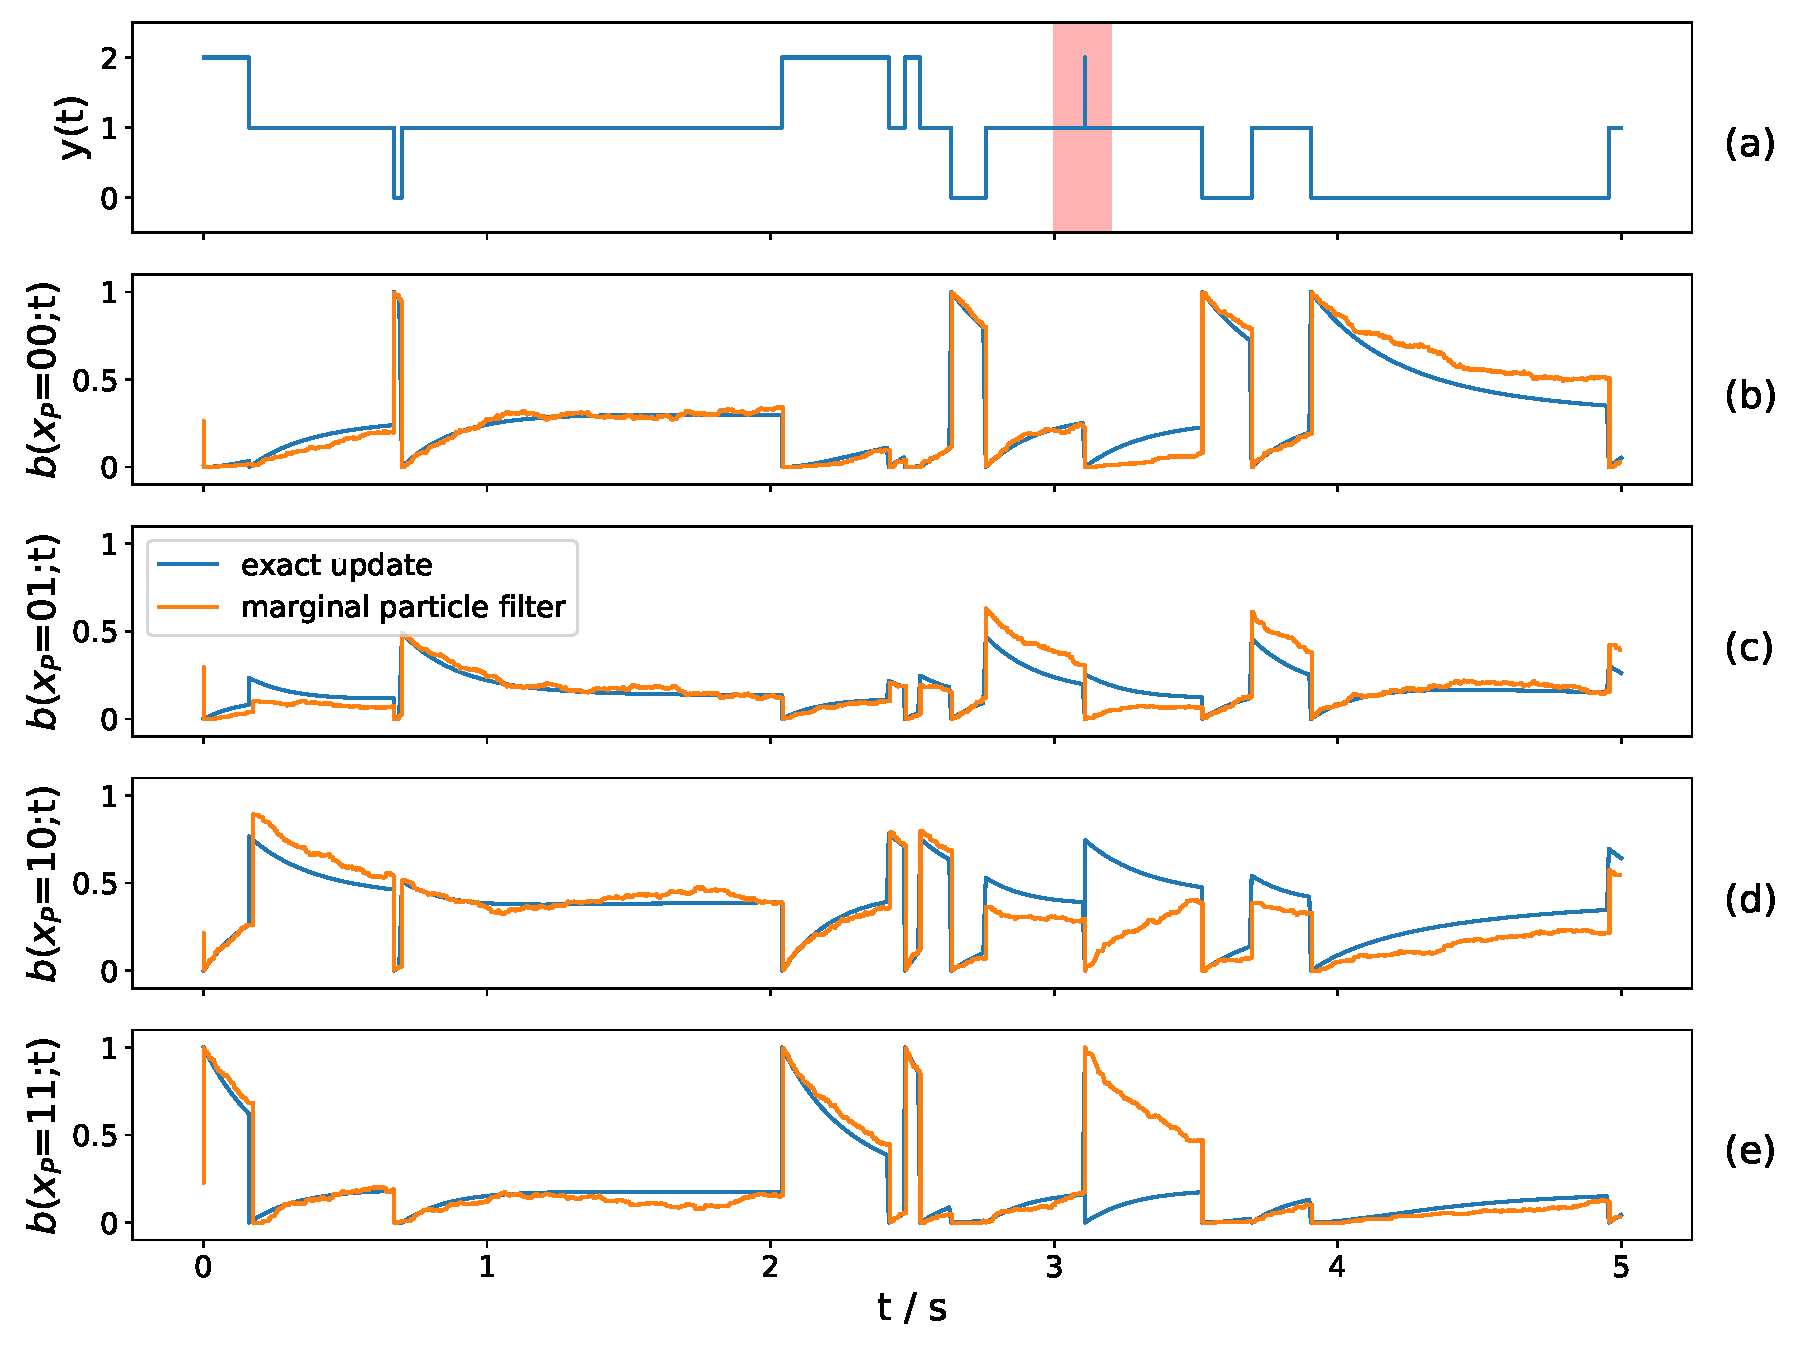
\includegraphics[width=.87\textwidth]{figures/degenerate_pf/belief_traj}
		\caption[Degenerate marginal particle filter]{A sample with degenerate marginal particle filter. The unlikely observation which has caused the degeneration is highlighted in (a). It can be seen in (d) and (e) that this observation causes particle filter approximation to diverge from exact update results but it is recovered with the next observation.}
		\label{fig:deg_partFilter}
	\end{center}
\end{figure}

\section{Inference of Observation Model}
We considered the problem of inferring the observation model as a classification problem. As a measure of the performance of the classifier, we utilised area under the Reciever-Operator-Characteristic curve (AUROC) and Presition-Recall curve (AUPR). 
\subsection{Equivalence Classes}
\label{sec:eq_classes}
As mentioned in \cref{sec:inf_setup}, the deterministic nature of the observation model results in a number of possible observation models. The setting described in \cref{chap:3} with configurations given in \cref{sec:config} leads to 81 obsevation models. However, with this experimental setup and the methods, it is only possible to distinguish these observation models into 10 different classes. Due to this equivalence, the inference problem is considered only for 10 observation models, each one representing one class. The reasons of this phenomena are discussed in detail in \cref{ap:eq_classes}, together with the observation models considered in the inference problem. The set of observation model that can be classified is denoted as $ \symbf{\psi} $ in the following. \\
\autoref{fig:llh_exactUpdate_81model} illustrates the equivalence of observation models clearly. The plot depicts the results of an experiment with 200 samples, $ |\xi_T| = 200 $, generated using the observation model $ \psi_{\text{true}} $ given in \cref{sec:config}, and the average log-likelihood of samples computed for all possible observation models. Here, the belief state is updated using exact method as described in \cref{par:bs_exact}, in order to depict the exact equivalence within one class. As can be seen, the results show the separation of the set of observation models into 10 distinct classes. The legend is removed to avoid clutter.
\begin{figure}[H]
	\begin{center}
		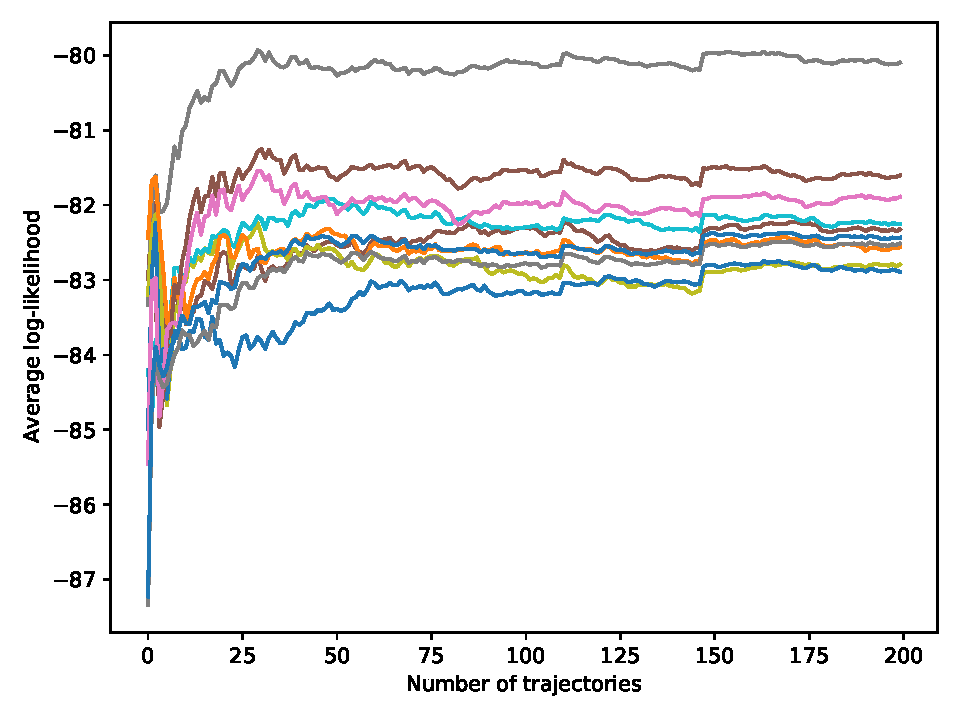
\includegraphics[width=.8\textwidth]{figures/equivalence_classes/llh_exactUpdate_81model}
		\caption[Equivalence classes in the case of exact belief update]{Average log-likelihood $ \log p(S^{[0,T]} \mid \theta) $ over samples generated using exact belief state update, depicting the equivalence classes in the set of observation models.}
		\label{fig:llh_exactUpdate_81model}
	\end{center}
\end{figure}
In order to show the validity of the equivalence in the case of marginal particle filter, the average log-likelihoods of 200 samples given two observation models in the same class are illustrated in \autoref{fig:llh_particleFilter_sameclass}. The samples are generated with $ \psi_{\text{true}} = \psi_{0} $, and the rest of the observation models here fall in the same equivalence class as $ \psi_0 $. As can be seen from the graph, the observation models lead to so similar results to each other that they are assumed to be identical. 
\begin{figure}[H]
	\begin{center}
		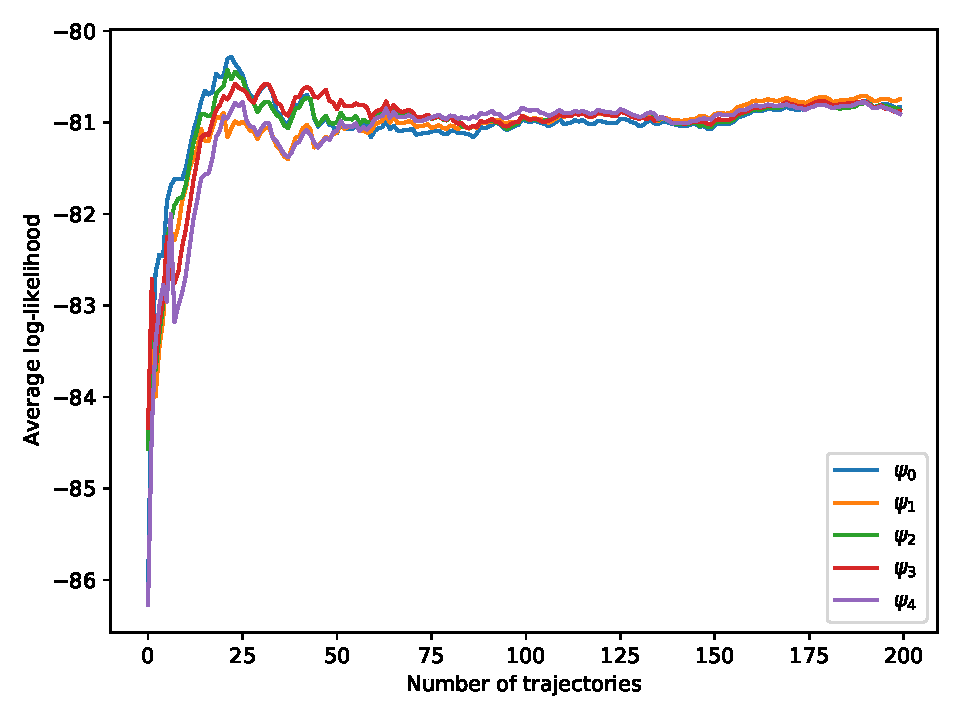
\includegraphics[width=.8\textwidth]{figures/equivalence_classes/llh_particleFilter_sameclass}
		\caption[An equivalence class in the case of marginal particle filtering]{Average log-likelihood $ \log p(S^{[0,T]} \mid \theta) $ over samples generated using marginal particle filtering, where $ \psi_1 $ and $ \psi_2 $ belongs in the same class.}
		\label{fig:llh_particleFilter_sameclass}
	\end{center}
\end{figure} 
\subsection{Learning Observation Model}
\autoref{fig:llh_exact} illustrates the average log-likelihood over 100 samples given the observation models. The samples are generated with $ \psi_{true} = \psi_0 $ given in \cref{sec:config}, and exact update method is utilised for belief state update. As can be seen, the curves converge quicly and the true model is well separated from others. Consequently, the maximum likelihood estimation by \autoref{eq:max_llh_est} leads to the correct result. \\
A similar experiment is documented in \autoref{fig:llh_particle}, where exact update method is replaced by marginal particle filtering. $ \psi_0 $ denotes the observation model that has generated the dataset, and it is correctly estimated as the true model. The jump around 50 trajectories can be explained by an encounter with a highly likely parent trajectories.
\begin{figure}[H]
	\begin{center}
		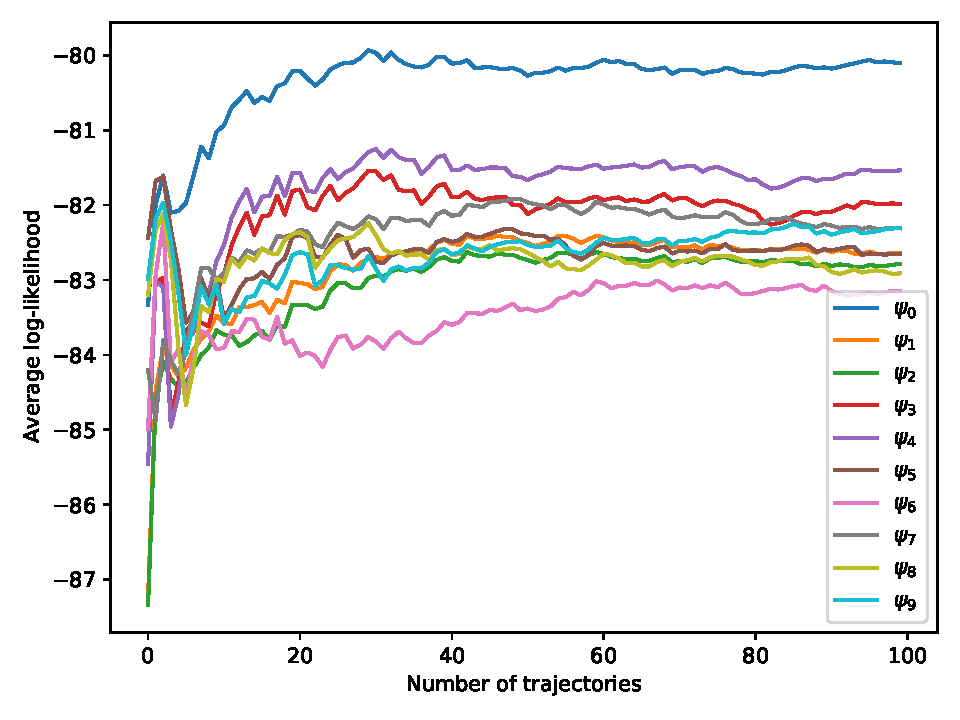
\includegraphics[width=.75\textwidth]{figures/roc_analysis/roc_exactUpdate/llh_exactUpdate_psi_0}
		\caption[Average log-likelihood in the case of exact belief update]{Average log-likelihood $ \log p(S^{[0,T]} \mid \theta) $ with $ \psi_i \in \symbf{\psi} $ over samples generated using exact belief state update}
		\label{fig:llh_exact}
	\end{center}
\end{figure}
\begin{figure}[H]
	\begin{center}
		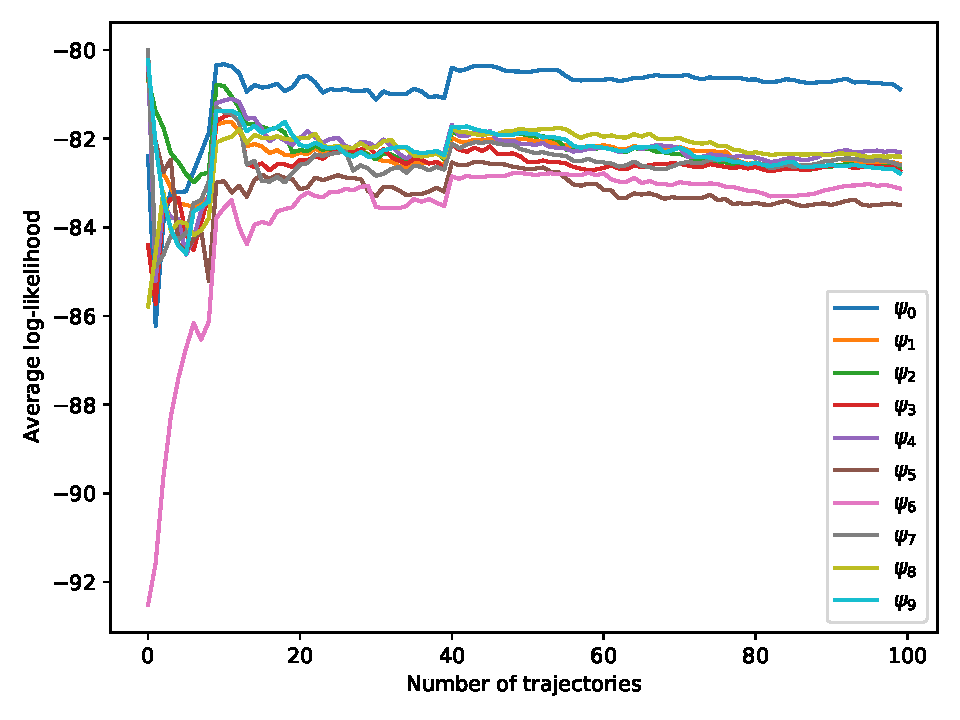
\includegraphics[width=.75\textwidth]{figures/roc_analysis/roc_particleFilter/llh_particleFilter_psi_0}
		\caption[Average log-likelihood in the case of marginal particle filtering]{Average log-likelihood $ \log p(S^{[0,T]} \mid \theta) $ with $ \psi_i \in \symbf{\psi} $ over samples generated using marginal particle filtering}
		\label{fig:llh_particle}
	\end{center}
\end{figure}
We approach the inference problem as classification between the observation models $ \psi \in \symbf{\psi} $ given in \cref{ap:obs_set_exp}. We consider the estimated likelihood values of each sample given an observation model as the score of the sample belonging to the corresponding class. Since this setting represents a multi-class classification problem, the
performance metrics AUROC and AUPR are calculated as one-vs-rest. \\ %performance metric AUROC is calculated as one-vs-rest. \\ %
Consider a binary classification problem. True positives (TP) are the samples predicted as 1 correctly, and false positives (FP) are the samples predicted as 1 while the true label was 0. True negatives (TN) are the samples predicted as 0 correctly, and false negatives (FN) are the samples with true label 1, but predicted 0. True positive rate (TPR), also called \textit{recall} (R) or \textit{sensitivity}, is the ratio of TPs over the number of samples which are labelled as 1. False positive rate (FPR) is the ratio of FPs over the number of samples labelled as 0. The precision (P) is the ratio of TPs over the number of all the samples predicted as 1.
\begin{align}
\text{TPR} = \text{R} &= \frac{\text{TP}}{\text{TP} + \text{FN}} \\
\text{FPR} &= \frac{\text{FP}}{\text{TN} + \text{FP}} \\
\text{P} &= \frac{\text{TP}}{\text{TP} + \text{FP}}
\end{align}
Receiver Operating Characteristics (ROC) curve illustrates the tradeoff between true positives and false positives, over different values of threshold for classification \cite{Robinson2008}. The area under ROC curve (AUROC) is a performance metric that shows how well the classifier can distinguish the classes. Higher AUROC metric indicates better performance, taking values in the interval [0,1]. Precision-Recall (PR) curve illustrates the relation between precision and recall, providing a metric to quantify how many of the predictions were correct \cite{Boyd2013}.\\
We provided the classifier with increasing number of samples for inference. This is achieved through bootstrapping a given number of trajectories, and using the mean likelihood over the bootrap batch as a new sample. The following AUROC plots shows the results over 50 trajectory generated using each obervation model as the true model. According to this, in our dataset, we have 500 trajectories, 50 from each class labelled through a vector with 10 entries, having only 1 for the true observation model and 0 for the rest. When number of trajectories is 1, each sample in the dataset considered individually. When number of trajectories is 2, within each class, 50 sample batches of size 2 are bootstrapped such that none of the batches consist of the same samples. By doing so, we keep the sample size at 50 per each class, regardless of the batch size. \\
\autoref{fig:AUROC_class0} shows the AUROC results over 10 runs, comparing the state estimator using exact update and marginal particle filtering. We plotted the median AUROC as a line and 25-75\% percentile as the shaded area. \autoref{fig:AUPR_class0} illustrates the AUPR in the same manner. As expected given the unbiased classifier, both metrics approach to 1 as the number of samples increases. Due to the stochasticity introduced by the marginal particle filtering as the state estimator, the results obtained with this method show slightly lower performance. 
%As expected given the unbiased classifier, this metric approaches to 1 as the number of samples increases. Due to the stochasticity introduced by the particle filtering as the state estimator, the results obtained with this method show slightly lower performance. 
\begin{figure}[H]
	\begin{center}
		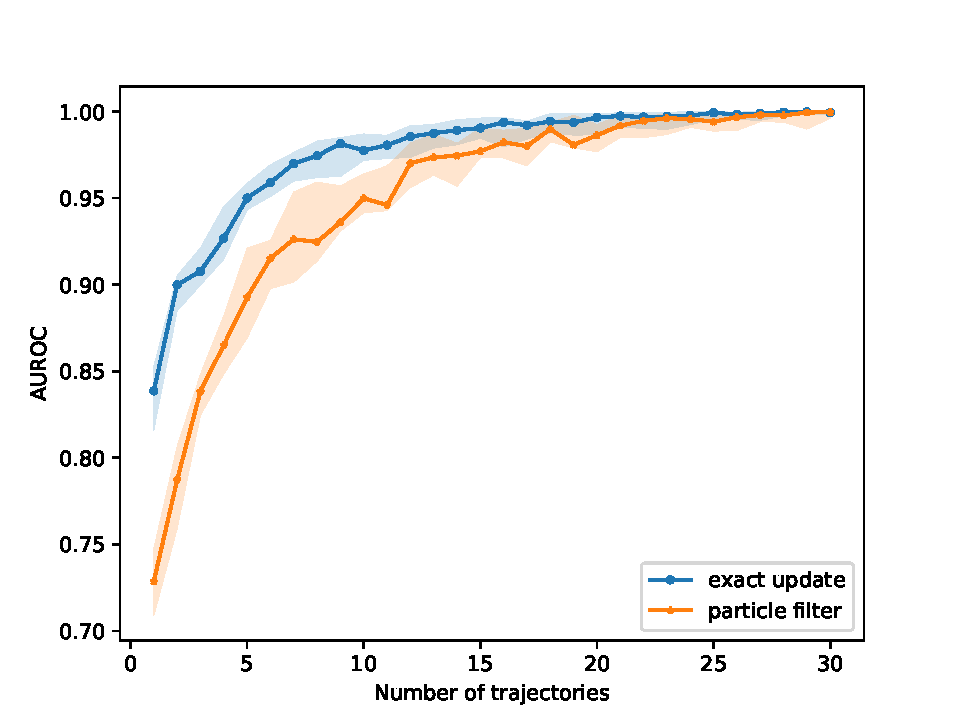
\includegraphics[width=.75\textwidth]{figures/roc_analysis/AUROC_perc_0}
		\caption[AUROC results over increasing number of samples]{AUROC results over increasing number of samples for $ \psi_0 $-vs-rest. We plotted the median with line and the 25-75\% percentile with the shaded area over 10 runs.}
		\label{fig:AUROC_class0}
	\end{center}
\end{figure}
\begin{figure}[H]
	\begin{center}
		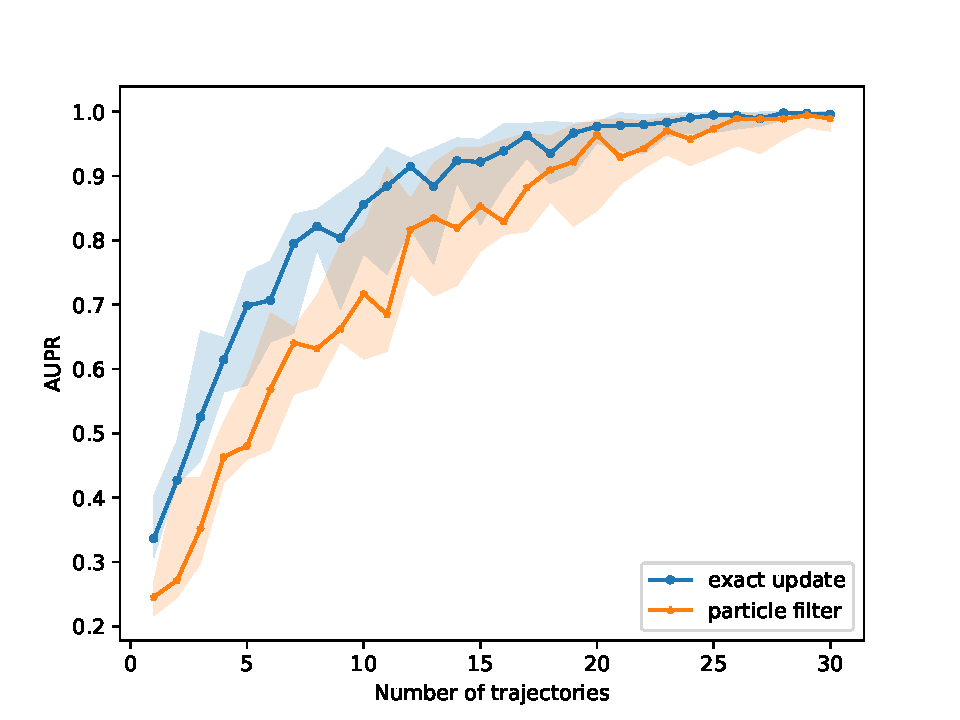
\includegraphics[width=.75\textwidth]{figures/roc_analysis/AUPR_perc_0}
		\caption[AUPR results over increasing number of samples]{AUPR results over increasing number of samples for $ \psi_0 $-vs-rest. We plotted the median with line and the 25-75\% percentile with the shaded area over 10 runs.}
		\label{fig:AUPR_class0}
	\end{center}
\end{figure}
\subsection{Inference with Non-informative Priors on Parent Parameters}
\begin{figure}[H]
	\begin{center}
		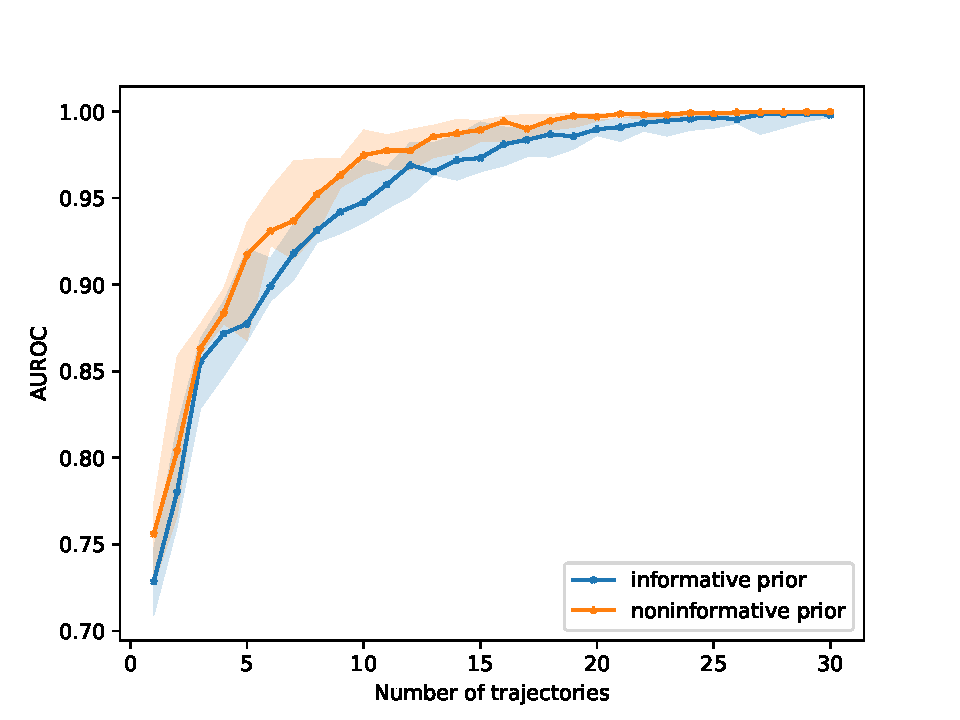
\includegraphics[width=.75\textwidth]{figures/roc_analysis/prior_AUROC_perc_0}
		\caption[AUROC results over increasing number of samples with different priors]{AUROC results over increasing number of samples for $ \psi_0 $-vs-rest. We plotted the median with line and the 25-75\% percentile with the shaded area over 10 runs.}
		\label{fig:AUROC_class0_prior}
	\end{center}
\end{figure}

\subsection{Robustness Test under Channel Noise}
\begin{figure}[H]
	\begin{center}
		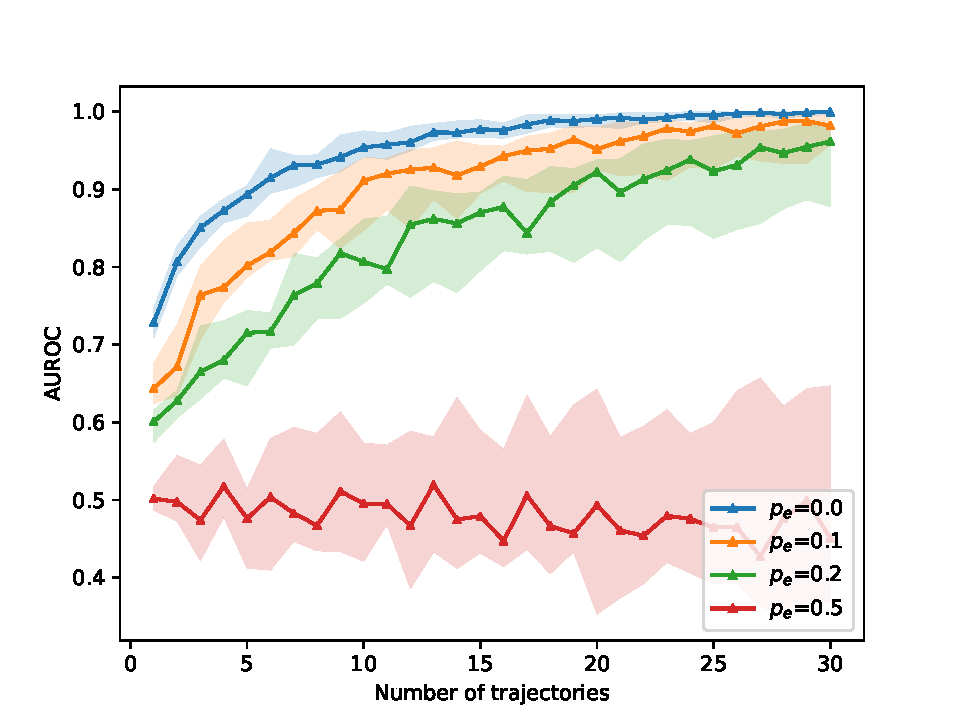
\includegraphics[width=.75\textwidth]{figures/roc_analysis/error_AUROC_perc_0}
		\caption[AUROC results over increasing number of samples with levels of noise]{AUROC results over increasing number of samples for $ \psi_0 $-vs-rest. We plotted the median with line and the 25-75\% percentile with the shaded area over 10 runs.}
		\label{fig:AUROC_class0_error}
	\end{center}
\end{figure}

	\newpage \ \thispagestyle{empty} \addtocounter{page}{-1}
	\chapter{Discussion}
\label{chap:5}
Motivated by the examples of multi-agent systems in nature, we modelled a communication between two parent nodes and an agent node combining CTBN and POMDP frameworks. While the parent nodes emit messages containing information about their states, the agent observes a translation of these messages from which it needs to form its belief state and make desicions. The nodes evolve continously in time as components of a CTBN, modelled as in \cref{sec:exp_ctbn_model}. Given that the messages of the parent nodes are unavailable to the agent, the interaction between the parent nodes and the agent node is modelled as POMDP, as described in \cref{sec:exp_pomdp_model}. We infer the observation model from simulated trajectories of nodes. \\
The belief state is updated utilising two methods. The first one is exact update, discussed in \cref{par:bs_exact}, and assumes that the transition intensities of the parents $ \textbf{Q}_1 $ and $ \textbf{Q}_2 $ are available for both the agent and the classifier. However, due to the fact that this would not present a realistic system, particle filtering with marginalized CTBN is introduced as the state estimator. Here, both the agent and the classifier was able to perform the belief state update, given Gamma-priors of $ \textbf{Q}_1 $ and $ \textbf{Q}_2 $.\\
We consider this problem as classification between observation models and analyze the performance of the classifier in terms of the metrics AUROC and AUPR. The results are given in \autoref{fig:AUROC_class0} and \autoref{fig:AUPR_class0}, respectively. Using exact method to update the belief state, excellent performance is achieved for the classification task regarding AUROC metric. The stochasticity introduced by the marginal particle filtering results in a slightly lower performance, compared to the exact update method. Nevertheless, in both methods, as the number of samples increases, the metric approaches to 1, which is expected in the case of the unbiased classifier.\\
The results of the experiments with different levels of noise added to the observation model are given in \autoref{fig:AUROC_class0_error}. We assume that the noise level is available to the agent, and the likelihoods of noise free observation models are considered for classification. Thus, the noisy model parameters are not estimated. The performance decreases as the noise introduced to the true observation model increases. These results confirm the expectations, as the noise leads to less reliable observations for the agent. On the other hand, with the increasing number of trajectories the metric converges to 1, showing robustness.\\
An important limitation to the inference task is the equivalence classes as introduced in \cref{sec:eq_classes}. The set of observation models can be divided into 10 equivalence classes such that the likelihoods of a sample trajectory $ S^{[0,T]} $ given any observation model within one class are equal. This clearly limits the classifiers ability to determine the true model. Due to this limitation, the set of observation models is reduced to 10 observation models, each one representing an equivalence class. These observation models are given in \cref{ap:obs_set_exp}. Consequently, the result which states that the true observation model is $ \psi_i $ is equivalent to the one which states that the true observation model belongs to $ \text{i}^{\text{th}} $ equivalence class. As shown with examples in \cref{ap:eq_classes}, there are two reason behind this equivalence. The first reason can be specified as the equivalent effect of observation models on the belief state, which is inherent to the observation model structure. The second reason is that the different belief states might lead to the same behaviour. This case can intuitively be explained by the fact that the agent may not need to use all the information it has for decision making. This information loss limits the ability to infer what the agent has observed from its actions.\\

\chapter{Outlook}
\label{chap:6}
The first step in the future of this work is to eliminate the equivalence classes to be able to classify every observation model. This problem, to a certain extent, can be mitigated by joint inference of observation model and policy. The joint inference could be performed as a joint classification problem, where the combination of discrete values of these parameters are treated as classes. This is only feasible by defining appropriate constraints on the policy such that, as for the case of observation models in this work, the policy space is countable. Another approach is to use function approximation to learn the observation model and the policy jointly.\\ 

Another exiciting direction is to employ our method in different environments to get insights in the interactions of agents and environments. 
Foerster \textit{et al.} \cite{Foerster2016}\\

%Another exiciting direction is to solve the policy optimization problem, instead of assuming that the optimal policy is given. By doing so, it would be feasible to utilise the classification method for observation model described in this work, in real-world data, providing insights in the interactions of agents and environments.\\
Moreover, it would be interesting to apply our model and solution approach to a more complex environment to evaluate the performance further. For example, one could experiment with non-binary messages, or more than two parent nodes.\\
\vspace{-13pt}
\begin{wrapfigure}{r}{6cm}
	\begin{center}
		\vspace{-13pt}
		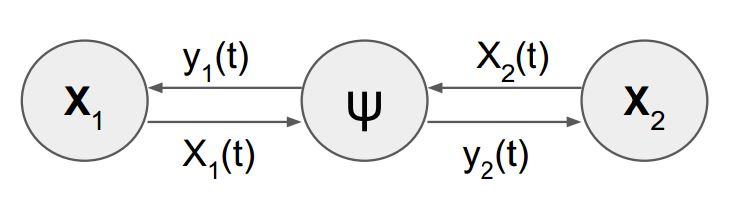
\includegraphics[width=5.5cm]{figures/multi-agent}
		\caption[Multi-agent communication model]{Multi-agent communication model.}
		\label{fig:multi_agent}
	\end{center}
\end{wrapfigure}
In this thesis, we assume that the messages are relevant for a single node, and its actions only affect itw own dynamics. An extension to this model is to consider bidirectional communication between agents, as depicted in \autoref{fig:multi_agent}. In such communication, both nodes send messages, which are translated by the same observation model, and their behaviour depends on their observations and the belief states they keep. 


	\bibliography{bib_cleaned}
	\addcontentsline{toc}{chapter}{Bibliography}
	\appendix\appendix

\chapter{Amalgamation}
\label{ap:amalgamation}
The amalgamation operation for two independent processes are derived as follows:
\begin{multline}
	\operatorname{Pr}(X_1(t+h) = x_1', X_2(t+h) = x_2 \mid X_1(t) = x_1, X_2(t) = x_2) \\
	\begin{split}
	&= \operatorname{Pr}(X_1(t+h) = x_1' \mid X_1(t) = x_1, X_2(t) = x_2) \operatorname{Pr}( X_2(t+h) = x_2 \mid X_1(t) = x_1, X_2(t+h) = x_2) \\
	& = (\delta_{x_1', x_1} + hq^1_{x_1, x_1^\prime} + o(h))(1 + hq^2_{x_2, x_2} + o(h))\\
	& = \delta_{x_1', x_1} + hq^1_{x_1, x_1^\prime} + h\delta_{x_1', x_1}q^2_{x_2, x_2} + o(h)
	\end{split}
	\label{eq:amalg}
\end{multline}



\chapter{Marginalized Likelihood Function for Homogenous Continuous Time Markov Processes}
\label{ap:marg_llh_ctmp}

Let $ X $ be a homogenous CTMP. For convenience, it is assumed to be binary-valued, $ \rchi = \left\lbrace x_{0}, x_{1} \right\rbrace $. The transition intensity matrix can be written in the following form:
\begin{equation}
\textbf{Q} = 
\begin{bmatrix}
-q_{0} & q_{0} \\
q_{1} & -q_{1}
\end{bmatrix}
\end{equation}
where the transition intensities $ q_{0} $ and $ q_{1} $ are gamma-distributed with parameters $ \alpha_{0}$, $ \beta_{0} $ and $ \alpha_{1} $, $ \beta_{1} $, respectively. The marginal likelihood of a sample trajectory $ X^{[0,T]} $ can be written as follows:
\begin{align}
P(X^{[0, T]}) & = \int  P(X^{[0, T]}\mid Q)P(Q) dQ \nonumber\\ 
& = \int_{0}^{\infty} = \prod_{j \neq i}  \exp(-q_{i,j}T[x_{i}])\ q_{i,j}^{M[x_{i},x_{j}]} \frac{\beta_{i,j}^{\alpha_{i,j}}{q_{i,j}^{\alpha_{i,j}-1}}\exp(-\beta_{i,j}q_{i,j})}{\Gamma(\alpha_{i,j})} \ dq_{i,j} \nonumber\\ 
& = \prod_{i\in{0,1}}\int_{0}^{\infty} q_{i}^{M[x_{i}]} \ \exp(-q_{i}T[x_{i}]) \  \frac{\beta_{i}^{\alpha_{i}} \ q_{i}^{\alpha_{i}-1}\ \exp(-\beta_{i}q_{i})}{\Gamma(\alpha_{i})} \ dq_{i} \nonumber\\ 
& = \prod_{i\in{0,1}} \frac{\beta_{i}^{\alpha_{i}}}{\Gamma(\alpha_{i})} \int_{0}^{\infty} q_{i}^{M[x_{i}] + \alpha_{i} -1} \ \exp(-q_{i}(T[x_{i}]+\beta_{i})) \ dq_{i} \label{eq:wolfram_line}\\ 
& = \prod_{i\in{0,1}} \frac{\beta_{i}^{\alpha_{i}}}{\Gamma(\alpha_{i})} \left( -(T[x_{i}]+\beta_{i})^{-M[x_{i}] - \alpha_{i}}\ \Gamma(M[x_{i}] + \alpha_{i}, \ q_{i}(T[x_{i}]+\beta_{i})) \right) \Big|_0^\infty  \nonumber\\ 
& = \prod_{i\in{0,1}} \frac{\beta_{i}^{\alpha_{i}}}{\Gamma(\alpha_{i})} \left( (T[x_{i}]+\beta_{i})^{-M[x_{i}] - \alpha_{i}}\ \Gamma(M[x_{i}] + \alpha_{i}) \right)
\label{eq:Marg_traj}
\end{align}
%where $ T[x_{i}] $, the amount of time spent in state x, $ M[x,x'] $ the number of transitions from state x to x' and  $ M[x] = \sum_{x\neq x'}M[x,x'] $.\\

In \autoref{eq:wolfram_line}, the integral is solved using computer algebra system WolframAlpha as follows:
\begin{align}
\int x^{a} \ \exp(-xb) \ dx = -b^{-a-1} \ \Gamma(a+1, \ bx) + C
\label{eq:integral}
\end{align}


\end{document}